%%%%%%%%%%%%%%%%%%%%%%%%%%%%%%%%%%%%%%%%%%%%%%%%%%%%%%%%%%%%%%%%%%%%
\section{Design}
\label{sec:fdsp-apa-design}

The physics performance of the \dword{spmod} is a function of many intertwined detector parameters including argon purity, drift distance, \efield, wire pitch, wire length, and noise levels in the readout \dword{ce}.  Energy deposits from \dwords{mip} originating anywhere inside the active volume of the detector should be identifiable with near \num{100}\% efficiency.  This requirement constrains aspects of the \dword{apa} design, specifically, the limits on wire pitch, wire length, and choice of wire material.  This section details the design of an individual \dword{apa}. We begin with an overview of the key fundamental parameters of the \dword{apa}s and their connection to the physics requirements of the \dword{dune} experiment. 


%%%%%%%%%%%%%%%%%%%%%%%%%%%%%%%%%%%%%%%%%%%%%%%%%%%%%%%%%%%%%%%%%%%%
\subsection{APA Design Parameters}
\label{sec:fdsp-apa-design-overview}

Each \dword{apa} is \SI{6}{m} high, \SI{2.3}{m} wide, and \SI{15}{cm} thick.  The underlying support frame is made from stainless steel hollow tube sections that are precisely machined and bolted together. A fine, conducting mesh covers the rectangular openings in the frame on both sides to define a uniform electrical \dword{gp} behind the wires. The four layers of sense and shielding wires at varying angles relative to each other completely cover the frame. The wires terminate on boards that anchor them as well as provide the electrical connection to the \dword{tpc} readout \dword{ce}. Starting from the outermost wire layer, there is first an uninstrumented shielding (grid) plane (strung vertically, $G$), followed by two induction planes (strung at \apainducwireangle to the vertical, $U,V$), and finally the collection plane (vertical, $X$). All wire layers span the full height of the \dword{apa} frame. The two planes of induction wires wrap in a helical fashion around the long edges and over both sides of the \dword{apa}. Figures~\ref{fig:tpc_apa1} and \ref{fig:sp-apa-head-xsec} illustrate the layout of the wire layers.  Below, we summarize the key design parameters and the considerations driving the main design choices for the \dword{apa}s.  A tabulated summary of \dword{apa} specific requirements is also provided in Table~\ref{tab:specs:SP-APA}.  


% This file is generated, any edits may be lost.

% It defines macros which expand to corresponding
% specification values for subsystem SP-APA



\begin{longtable}{p{0.14\textwidth}p{0.13\textwidth}p{0.18\textwidth}p{0.22\textwidth}p{0.20\textwidth}}
\caption{Specifications for SP-APA \fixmehl{ref \texttt{tab:spec:SP-APA}}} \\
  \rowcolor{dunesky}
       Label & Description  & Specification \newline (Goal) & Rationale & Validation \\  \colhline

   \newtag{SP-FD-1}{ spec:min-drift-field }  & Minimum drift field  &  $>$\,\SI{250}{ V/cm} \newline ( $>\,\SI{500}{ V/cm}$ ) &  Lessens impacts of $e^-$-Ar recombination, $e^-$ lifetime, $e^-$ diffusion and space charge. &  ProtoDUNE \\ \colhline
    
   
  \newtag{SP-FD-2}{ spec:system-noise }  & System noise  &  $<\,\SI{1000}\,e^-$ &  Provides $>$5:1 S/N on induction planes for  pattern recognition and two-track separation. &  ProtoDUNE and simulation \\ \colhline
    
   
  \newtag{SP-FD-3}{ spec:light-yield }  & Light yield  &  $>\,\SI{20}{PE/MeV}$ (avg), $>\,\SI{0.5}{PE/MeV}$ (min) &  Gives PDS energy resolution comparable that of the TPC for 5-7 MeV SN $\nu$s, and allows tagging of $>\,\SI{99}{\%}$ of nucleon decay backgrounds with light at all points in detector. &  Supernova and nucleon decay events in the FD with full simulation and reconstruction. \\ \colhline
    
    \\ \rowcolor{dunesky} \newtag{SP-FD-4}{ spec:time-resolution-pds } & Name: Time resolution \\
    Description & The time resolution of the photon detection system shall be less than 1 microsecond in order to assign a unique event time.   \\  \colhline
    Specification (Goal) &  $<\,\SI{1}{\micro\second}$  ( $<\,\SI{100}{\nano\second}$ ) \\   \colhline
    Rationale &   Enables \SI{1}{mm} position resolution for \SI{10}{MeV} SNB candidate events for instantaneous rate $<\,\SI{1}{m^{-3}ms^{-1}}$.  \\ \colhline
    Validation &   \\
   \colhline

   \newtag{SP-FD-5}{ spec:lar-purity }  & Liquid argon purity  &  $<$\,\SI{100}{ppt} \newline ($<\,\SI{30}{ppt}$) &  Provides $>$5:1 S/N on induction planes for  pattern recognition and two-track separation. &  Purity monitors and cosmic ray tracks \\ \colhline
    
    \\ \rowcolor{dunesky} \newtag{SP-FD-6}{ spec:apa-gaps } & Name: Gaps between APAs  \\
    Description & The gap size between APAs shall minimize loss of fiducial volume and distortion of charge collection.   \\  \colhline
    Specification &  $<\,\SI{15}{mm}$ between APAs on same support beam; $<\,\SI{30}{mm}$ between APAs on different support beams \\   \colhline
    Rationale &   Maintains fiducial volume.  Simplified contruction.  \\ \colhline
    Validation & ProtoDUNE  \\
   \colhline

    \\ \rowcolor{dunesky} \newtag{SP-FD-7}{ spec:misalignment-field-uniformity } & Name: Drift field uniformity due to component alignment \\
    Description & Misalignments of the various TPC components shall not introduce drift-field nonuniformities beyond those specified in the HVS requirements.   \\  \colhline
    Specification &  $<\,1\,$\% throughout volume \\   \colhline
    Rationale &   Maintains APA, CPA,  FC orientation and shape.  \\ \colhline
    Validation & ProtoDUNE  \\
   \colhline

    
   
  \newtag{SP-FD-8}{ spec:apa-wire-angles }  & APA wire angles  &  \SI{0}{\degree} for collection wires, \SI{35.7}{\degree} for induction wires &  Minimize inter-APA dead space. &  Engineering calculation \\ \colhline
    
    
   
  \newtag{SP-FD-9}{ spec:apa-wire-spacing }  & APA wire spacing  &  \SI{4.669}{mm} for U,V; \SI{4.790}{mm} for X,G &  Enables 100\% efficient MIP detection, \SI{1.5}{cm} $yz$ vertex resolution. &  Simulation \\ \colhline
    
   
  \newtag{SP-FD-10}{ spec:apa-wire-pos-tolerance }  & APA wire position tolerance  &  $\pm\,\SI{0.5}{mm}$ &  Interplane electron transparency; $dE/dx$, range, and MCS calibration. &  ProtoDUNE and simulation \\ \colhline
    

    \\ \rowcolor{dunesky} \newtag{SP-APA-1}{ spec:apa-unit-size } & Name: APA unit size \\
    Description & Overall dimensions of a single anode plane assembly   \\  \colhline
    Specification &  \SI{6.0}{m} tall $\times$ \SI{2.3}{m} wide \\   \colhline
    Rationale &   Maximum size allowed for fabrication, transportation, and installation.   \\ \colhline
    Validation & ProtoDUNE-SP   \\
   \colhline

   
  \newtag{SP-APA-2}{ spec:apa-active-area }  & Active area  &  Maximize total active area. &  Maximize area for data collection  &  ProtoDUNE-SP  \\ \colhline
    
   
  \newtag{SP-APA-3}{ spec:apa-wire-tension }  & Wire tension  &  \SI{6}{N} $\pm$ \SI{1}{N} &  Prevent contact beween wires and minimize  break risk &  ProtoDUNE-SP \\ \colhline
    
    \\ \rowcolor{dunesky} \newtag{SP-APA-4}{ spec:apa-bias-voltage } & Name: Wire plane bias voltages \\
    Description & APAs should produce optimal and uniform induction and collection signal shapes.   \\  \colhline
    Specification &  The setup, including boards, must hold 150\% of max operating voltage. \\   \colhline
    Rationale &   Headroom in case adjustments needed  \\ \colhline
    Validation & E-field simulation sets wire bias voltages. ProtoDUNE-SP confirms performance.  \\
   \colhline

    
   
  \newtag{SP-APA-5}{ spec:apa-frame-planarity }  & Frame planarity (twist limit)  &  $<$\SI{5}{mm} &  APA transparency.  Ensures wire plane spacing change of $<$0.5 mm.  &  ProtoDUNE-SP \\ \colhline
    
    
   
  \newtag{SP-APA-6}{ spec:apa-bad-channels }  & Missing/unreadable channels  &  $<$1\%, with a goal of $<$0.5\% &  Reconstruction efficiency &  ProtoDUNE-SP \\ \colhline
    


\label{tab:specs:SP-APA}
\end{longtable}
%% This file is generated, any edits may be lost.

% It defines macros which expand to corresponding
% specification values for subsystem SP-APA



\begin{longtable}{p{0.13\textwidth}p{0.15\textwidth}p{0.22\textwidth}p{0.25\textwidth}p{0.18\textwidth}}    

\caption{Specifications for SP-APA \fixmehl{ref \texttt{tab:specs:SP-APA}}} \\

\rowcolor{dunesky}
  Label & Name  & Specification \newline (Goal) & Rationale & Validation \\  \colhline

  \newtag{SP-FD-1}{ spec:min-drift-field }  & Minimum drift field  &  $>$\,\SI{250}{ V/cm} \newline ( $>\,\SI{500}{ V/cm}$ ) &  Lessens impacts of e-Ar recombination, e-lifetime, e-diffusion and space charge. &  ProtoDUNE \\ \colhline
    
 
 \newtag{SP-FD-2}{ spec:system-noise }  & System noise  &  $<\,\SI{1000}{enc}$ &  Provides $>$5:1 S/N on induction planes for  pattern recognition and two-track separation. &  ProtoDUNE and simulation \\ \colhline
 
   \newtag{SP-FD-3}{ spec:light-yield }  & Light yield  &  $>\,\SI{0.5}{pe/MeV}$ \newline ( $>\,\SI{5}{pe/MeV}$ ) &  Rejects nucleon decay backgrounds from cosmogenic events near cathode. &   \\ \colhline
  
 \newtag{SP-FD-4}{ spec:time-resolution-pds }  & Time resolution  &  $<\,\SI{1}{\micro\second}$ \newline ( $<\,\SI{100}{\nano\second}$ ) &  Enables \SI{1}{mm} position resolution for \SI{10}{MeV} SNB candidate events for instantaneous rate $<\,\SI{1}{m^{-3}ms^{-1}}$. &   \\ \colhline
 
 
   \newtag{SP-FD-5}{ spec:lar-purity }  & Liquid argon purity  &  $<$\,\SI{100}{ppt} \newline ( $<\,\SI{30}{ppt}$ ) &  Provides $>$5:1 S/N on induction planes for  pattern recognition and two-track separation. &  Purity monitors and cosmic ray tracks \\ \colhline
    

 \newtag{SP-FD-6}{ spec:apa-gaps }  & Gaps between APAs   &  $<\,\SI{15}{mm}$ between APAs on same support beam; $<\,\SI{30}{mm}$ between APAs on different support beams &  Maintains fiducial volume.  Simplified contruction. &  ProtoDUNE \\ \colhline

 \newtag{SP-FD-7}{ spec:misalignment-field-uniformity }  & Drift field uniformity due to component alignment  &  $<\,1\,$\% throughout volume &  Maintains APA, CPA,  FC orientation and shape. &  ProtoDUNE \\ \colhline
   
  \newtag{SP-FD-8}{ spec:apa-wire-angles }  & APA wire angles  &  \SI{0}{\degree} for collection wires, \SI{35.7}{\degree} for induction wires &  Minimize inter-APA dead space. &  Engineering calculation \\ \colhline
   
   \newtag{SP-FD-9}{ spec:apa-wire-spacing }  & APA wire spacing  &  \SI{4.669}{mm} for U,V; \SI{4.790}{mm} for X,G &  Enables 100\% efficient MIP detection, \SI{1.5}{cm} $yz$ vertex resolution. &  Simulation \\ \colhline
   
   \newtag{SP-FD-10}{ spec:apa-wire-pos-tolerance }  & APA wire position tolerance  &  $\pm\,\SI{0.5}{mm}$ &  Interplane electron transparency; $dE/dx$, range, and MCS calibration. &  ProtoDUNE and simulation \\ \colhline
    
 % \newtag{SP-APA-1}{ spec:apa-unit-size }  & Overall dimensions of a single anode plane assembly  &  \SI{6.0}{m} tall $\times$ \SI{2.3}{m} wide &  Maximum size allowed for fabrication, transportation, and installation.  &  ProtoDUNE-SP  \\ \colhline
    \newtag{SP-APA-1}{ spec:apa-unit-size }  & APA unit size  &  \SI{6.0}{m} tall $\times$ \SI{2.3}{m} wide &  Maximum size allowed for fabrication, transportation, and installation.  &  ProtoDUNE-SP  \\ \colhline 
    

%  \newtag{SP-APA-2}{ spec:apa-active-area }  & APAs should be sensitive over most of the full area of an APA frame, limiting dead regions in the detector volume.  &  Maximize total active area. &  Maximize area for data collection  &  ProtoDUNE-SP  \\ \colhline
 \newtag{SP-APA-2}{ spec:apa-active-area }  & Active area  &  Maximize total active area. &  Maximize area for data collection  &  ProtoDUNE-SP  \\ \colhline
    
    

 % \newtag{SP-APA-3}{ spec:apa-wire-tension }  & APA wires shall not touch during operation and break risk must be kept to a minimum.   &  \SI{6}{N} $\pm$ \SI{1}{N} &  Prevent contact beween wires and minimize  break risk &  ProtoDUNE-SP \\ \colhline
     \newtag{SP-APA-1}{ spec:apa-unit-size }  & APA unit size  &  \SI{6.0}{m} tall $\times$ \SI{2.3}{m} wide &  Maximum size allowed for fabrication, transportation, and installation.  &  ProtoDUNE-SP  \\ \colhline

%  \newtag{SP-APA-4}{ spec:apa-bias-voltage }  & APAs should produce optimal and uniform induction and collection signal shapes.  &  The setup, including boards, must hold 150\% of max operating voltage. &  Headroom in case adjustments needed &  E-field simulation sets wire bias voltages. ProtoDUNE-SP confirms performance. \\ \colhline
 \newtag{SP-APA-4}{ spec:apa-bias-voltage }  & Wire plane bias voltages  &  The setup, including boards, must hold 150\% of max operating voltage. &  Headroom in case adjustments needed &  E field simulation sets wire bias voltages. ProtoDUNE-SP confirms performance. \\ \colhline    
    

%  \newtag{SP-APA-5}{ spec:apa-frame-planarity }  & Overall twist of the APA frame.  &  $<$\SI{5}{mm} &  APA transparency.  Ensures wire plane spacing change of $<$0.5 mm.  &  ProtoDUNE-SP \\ \colhline
  \newtag{SP-APA-5}{ spec:apa-frame-planarity }  & Frame planarity (twist limit)  &  $<$\SI{5}{mm} &  APA transparency.  Ensures wire plane spacing change of $<$0.5 mm.  &  ProtoDUNE-SP \\ \colhline  
    

%  \newtag{SP-APA-6}{ spec:apa-bad-channels }  & Number of channels incapable of recording signals.  &  $<$1\%, with a goal of $<$0.5\% &  Reconstruction efficiency &  ProtoDUNE-SP \\ \colhline
     \newtag{SP-APA-6}{ spec:apa-bad-channels }  & Missing/ unreadable channels  &  $<$1\%, with a goal of $<$0.5\% &  Reconstruction efficiency &  ProtoDUNE-SP \\ \colhline
    
\label{tab:SP-APA-specs}

\end{longtable}  %need to replace; anne 1/8

\begin{itemize}
\item \textbf{\dword{apa} size:} The size of the \dword{apa}s is chosen for fabrication purposes, compatibility with over-the-road shipping, and for eventual transport to the 4,850L at \dword{surf} and installation into %the membrane cryostat of a \dword{detmodule}. 
a cryostat. The dimensions are also chosen so that an integral number of electronic readout channels and boards instrument the full area of the \dword{apa}.

\item \textbf{Detector active area:} \dword{apa}s should be sensitive over most of the full area of an \dword{apa} frame, with any dead regions between \dword{apa}s due to frame elements, wire boards, electronics, or cabling kept to a minimum.  The wrapped style shown in Figure~\ref{fig:tpc_apa1} allows all channels to be read out at the top of the \dword{apa}, eliminating the dead space between \dword{apa}s that would otherwise be created by electronics and associated cabling. In addition, in the design of the \dword{spmod}, a central row of 
\dword{apa}s is flanked by drift-field regions on either side (Figure~\ref{fig:DUNESchematic1ch1}), %(see Figure~\ref{fig:FarDet-interior}), 
and the wrapped design allows the induction plane wires to sense drifted ionization that originates from either side of the \dword{apa}.  This double-sided feature is also effective for the \dword{apa}s located against the cryostat walls where the drift field is on only one side; the grid layer facing the wall effectively blocks any ionization generated outside the \dword{tpc} from drifting in to the wires on that side of the \dword{apa}.        

\item \textbf{Wire angles:} The $X$ wires run vertically to provide optimal reconstruction of beam-induced particle tracks, which are predominantly forward (in the beam direction). The angle of the induction planes on the \dword{apa}, \apainducwireangle, was chosen to ensure that each induction wire only crosses a given collection wire once, reducing the ambiguities that the reconstruction must address.  Simulation studies (see next item) show that this configuration performs similarly to an optimal 45$^\circ$ wire angle for the primary \dword{dune} physics channels.  The design angle of the induction wires, coupled with their pitch, also satisfies the requirement %that an integer multiple of electronics boards be needed to read out one \dword{apa}.
of using an integer multiple of electronics boards to read out one \dword{apa}.

\item \textbf{Wire pitch:} The wire spacing, \xgpitch for $(X,G)$ and \uvpitch for $(U,V)$, combined with key parameters for other \dword{tpc} systems %(described in their respective sections of the \dword{tdr}), 
can achieve the required performance for energy deposits by \dwords{mip} while providing good tracking resolution and good granularity for particle identification. The \single requirement that it be possible to determine the fiducial volume to \num{1}\% implies a vertex resolution of \SI{1.5}{cm} along each coordinate direction. The $\sim$\SI{4.7}{mm} wire pitch achieves this for the $y$ and $z$ coordinates.  The resolution on $x$, the drift coordinate, will be better than in the $y$--$z$ plane because of the combination of drift velocity and electronics sampling rate.  Finally, as already mentioned, the total number of wires on an \dword{apa} will match the granularity of the electronics boards (each \dword{femb} can read out \num{128} wires, mixed between the $U,V,X$ planes). This determines the exact wire spacings of \xgpitch on the collection plane and \uvpitch on the induction planes.  To achieve the reconstruction precision required (e.g., for $dE/dx$ reconstruction accuracy and multiple Coulomb scattering determination), the tolerance on the wire pitch is \wirepitchtol.

In 2017, the \dword{dune} \dword{fd} task force, using a full \dword{fd} simulation and reconstruction chain, performed detector optimization studies to quantify the impact of design choices, including wire pitch and wire angle, on \dword{dune} physics performance.  The results indicated that reducing wire spacing (to \SI{3}{mm}) or changing wire angle (to \num{45}$^\circ$) would not significantly affect the performance for the main physics goals of \dword{dune}, including $\nu_\mu $ to $\nu_e$ oscillations and \dword{cpv} sensitivity.  
A key low-level metric for oscillation physics is the ability to distinguish electrons versus photons in the detector because photon induced showers can fake electron showers and create \dword{nc} generated backgrounds in the $\nu_e$ \dword{cc} event sample.  Two important handles for reducing this contamination are (1)~the visible gap between the vertex of the neutrino interaction and the start of a photon shower, and %(2)~the energy density at the start of the shower being consistent with one \dword{mip} instead of two.  
(2)~the accordance of the energy density at the start of the shower with one \dword{mip} instead of two.

\begin{dunefigure}[Electron-photon separation dependence on wire pitch and angle]{fig:e-gamma}
{Summary of electron--photon separation performance studies from the \dword{dune} \dword{fd} task force. (a) $e$--$\gamma$ separation by $dE/dx$ for the nominal wire spacing and angle (\SI{4.7}{mm}/$37.5^\circ$) compared to \SI{3}{mm} spacing or 45$^\circ$ induction wire angles. (b) Electron signal selection efficiency versus photon (background) rejection for the different detector configurations. The \SI{3}{mm} wire pitch and 45$^\circ$ wire angle have similar effects, so the 45$^\circ$ curve is partly obscured by the \SI{3}{mm} curve.}
(a)
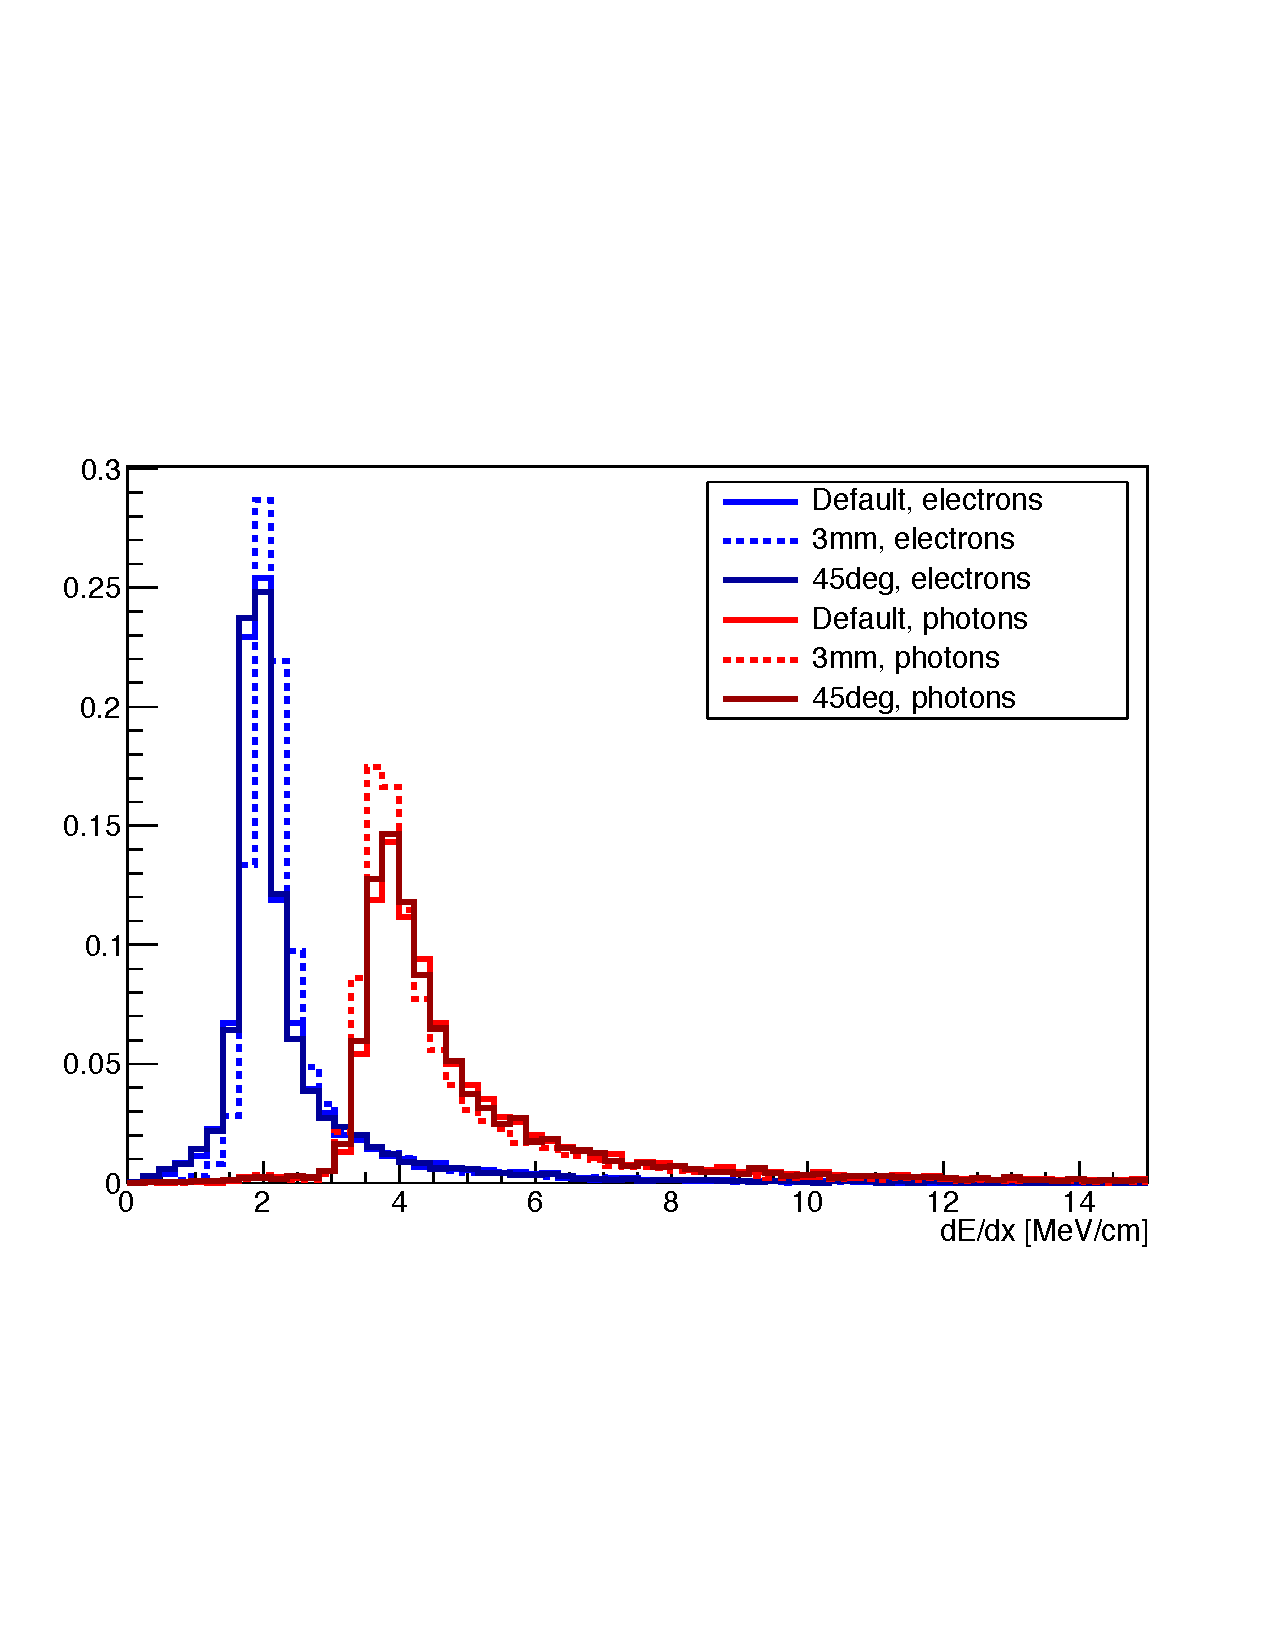
\includegraphics[height=0.24\textheight]{sp-apa-e-gamma-dEdx.pdf} \qquad
(b)
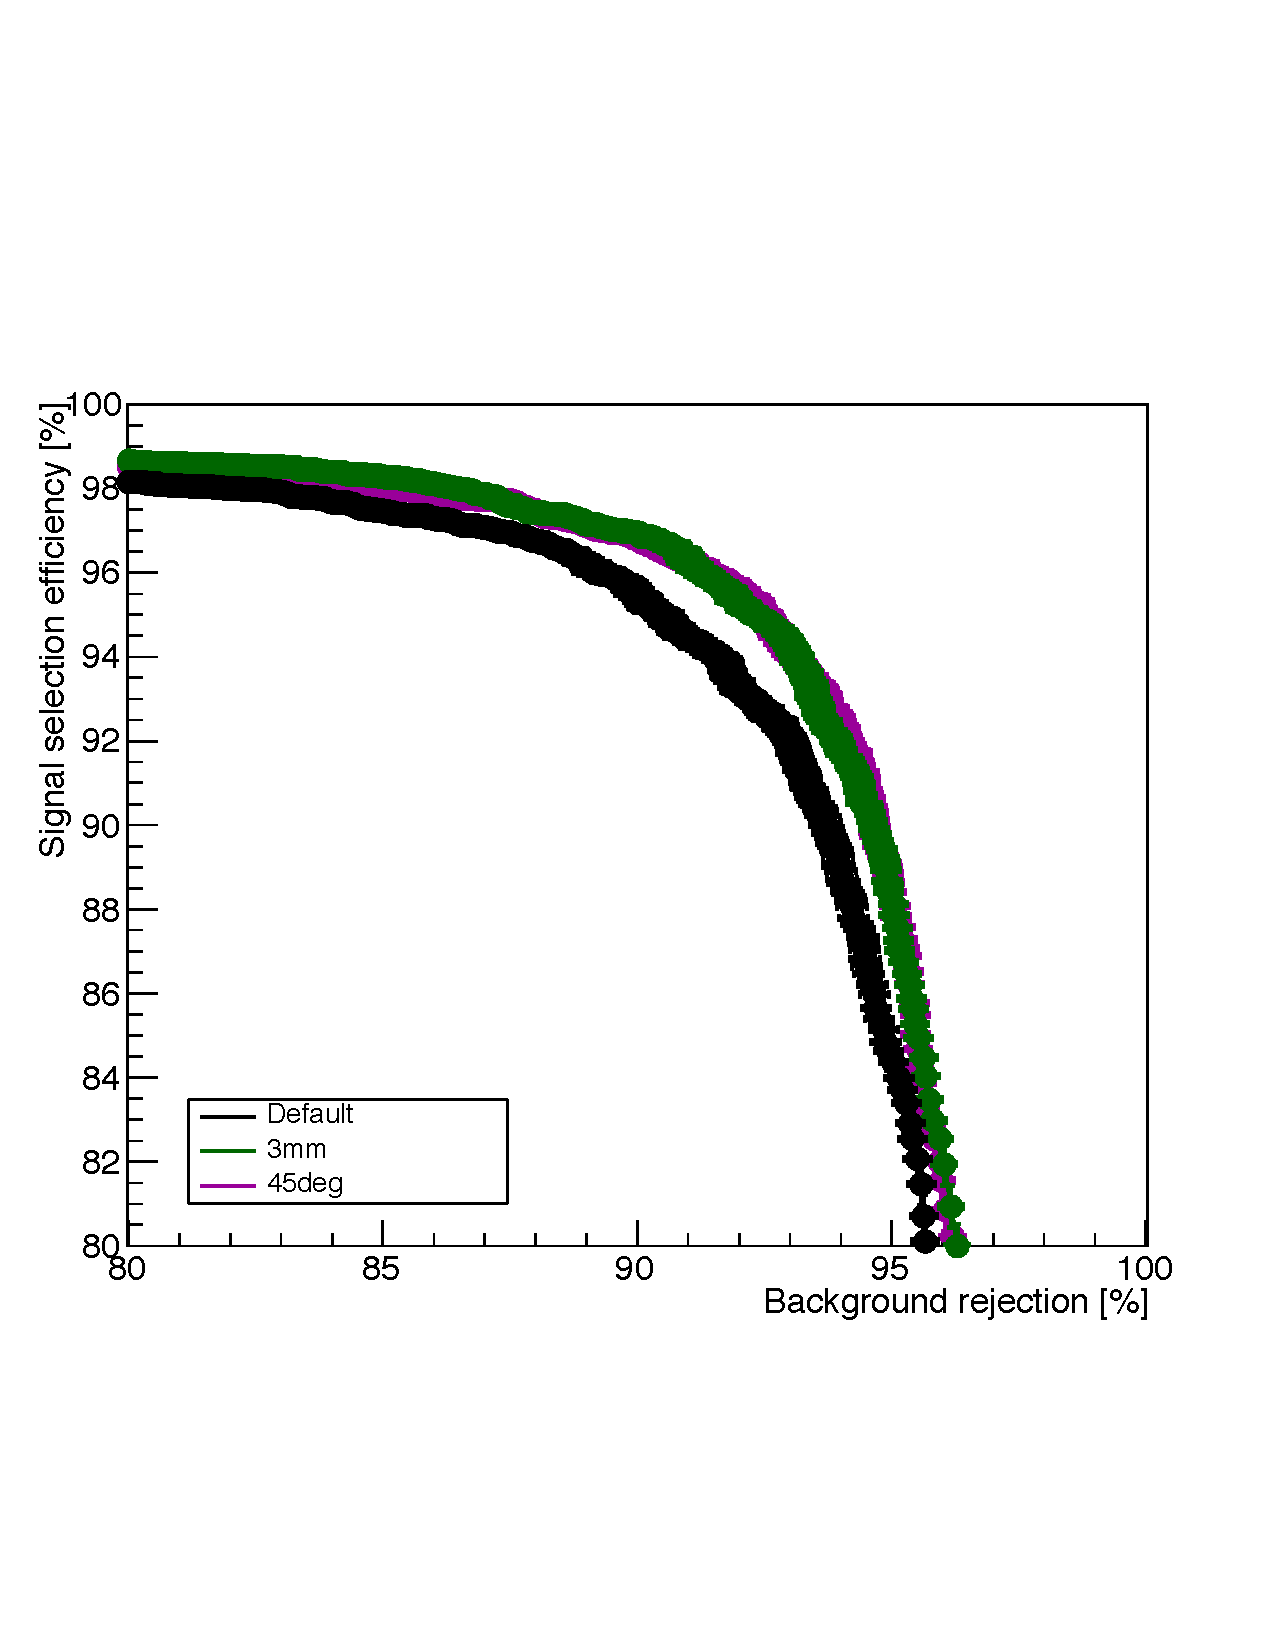
\includegraphics[height=0.24\textheight]{sp-apa-eff-bkgd-wires.pdf} 
\end{dunefigure}

A detector spatial resolution much smaller than the radiation length for photons (\SI{0.47}{cm} vs. \SI{14}{cm}) allows the gap between the neutrino interaction vertex and a photon conversion point to be easily visible, and  Figure~\ref{fig:e-gamma}(a) shows the reconstructed ionization energy loss density ($dE/dx$) in the first centimeters of electron and photon showers, illustrating the separation between the single \dword{mip} signal from electrons and the double \dword{mip} signal when photons pair-produce an $e^+e^-$.  In the figure, the ($dE/dx$) separation for electrons and photons is compared for finer wire pitch (\SI{3}{mm}) and optimal wire angle ($45^\circ$). The final electron signal selection efficiency is also shown as a function of the background rejection rate for different wire configurations in Figure~\ref{fig:e-gamma}(b). At a signal efficiency of \num{90}\,\%, for example, the background rejection can be improved by about \num{1}\,\% using either \SI{3}{mm} spacing or 45$^\circ$ wire angles for the induction planes.  This slight improvement in background rejection with more dense hit information or more optimal wire angles is not surprising, but the effect on high-level physics sensitivities from these changes is very small. The conclusions of the \dword{fd} task force, therefore, were that the introduction of ambiguities into the reconstruction by increasing the wire angles is not a good trade off, and the increase in cost incurred by decreasing the wire pitch (and, therefore, increasing the number of readout channels) is not justified.  



\item \textbf{Wire plane transparency and signal shapes:}  The ordering of the layers, starting from the active detector region, is $G$-$U$-$V$-$X$, followed by the grounding mesh. The operating voltages of the \dword{apa} layers are listed in Table~\ref{tab:bias}.  These were calculated by COMSOL software %~\cite{COMSOL} 
in order to maintain a \num{100}\% ionization electron transparency as they travel through the grid and induction wire planes. Figure~\ref{fig:apa-fields} shows the field simulation and expected signal shapes for the bias voltages listed in the table.  When operated at these voltages, the drifting ionization follows trajectories around the grid and induction wires, terminating on a collection plane wire. The grid and induction layers are completely transparent to drifting ionization, and the collection plane is completely opaque.  The grid layer is present for pulse-shaping and not connected to the electronics readout; it effectively shields the first induction plane from the drifting charge and removes a long leading edge from the signals on that layer.  These operating conditions were confirmed by a set of dedicated runs in \dword{pdsp} taken with various bias voltage settings during spring 2019 (see Sec.~\ref{sec:fdsp-apa-qa-protodune-ops} for a detailed discussion).

\begin{dunetable}[APA wire plane nominal bias voltages]{lr}{tab:bias}
{Baseline bias voltages for \dword{apa} wire layers for a 100\% ionization electron transparency as they travel through the grid and induction wire planes. These values were calculated by COMSOL software %~\cite{COMSOL} 
and confirmed by analytical calculations based on the conformal representation theory as well as dedicated data from \dword{pdsp}.} 
\textbf{Anode Plane} & \textbf{Bias Voltage} \\ \toprowrule
$G$ - Grid & \SI{-665}{V} \\ \colhline
$U$ - Induction & \SI{-370}{V{}} \\ \colhline
$V$ - Induction & \SI{0}{V} \\ \colhline
$X$ - Collection & \SI{820}{V} \\ \colhline
Grounding Mesh & \SI{0}{V} \\ 
\end{dunetable}

\begin{dunefigure}[Field line simulation around wire planes]{fig:apa-fields}
{Field lines (a) and resulting signal shapes on the APA induction and collection wires (b) according to a 2D electric field simulation.  The bi-polar nature of the induced signals on the $U$ and $V$ wires together with the uni-polar collection signals on $Y$ are clearly illustrated.}
a) 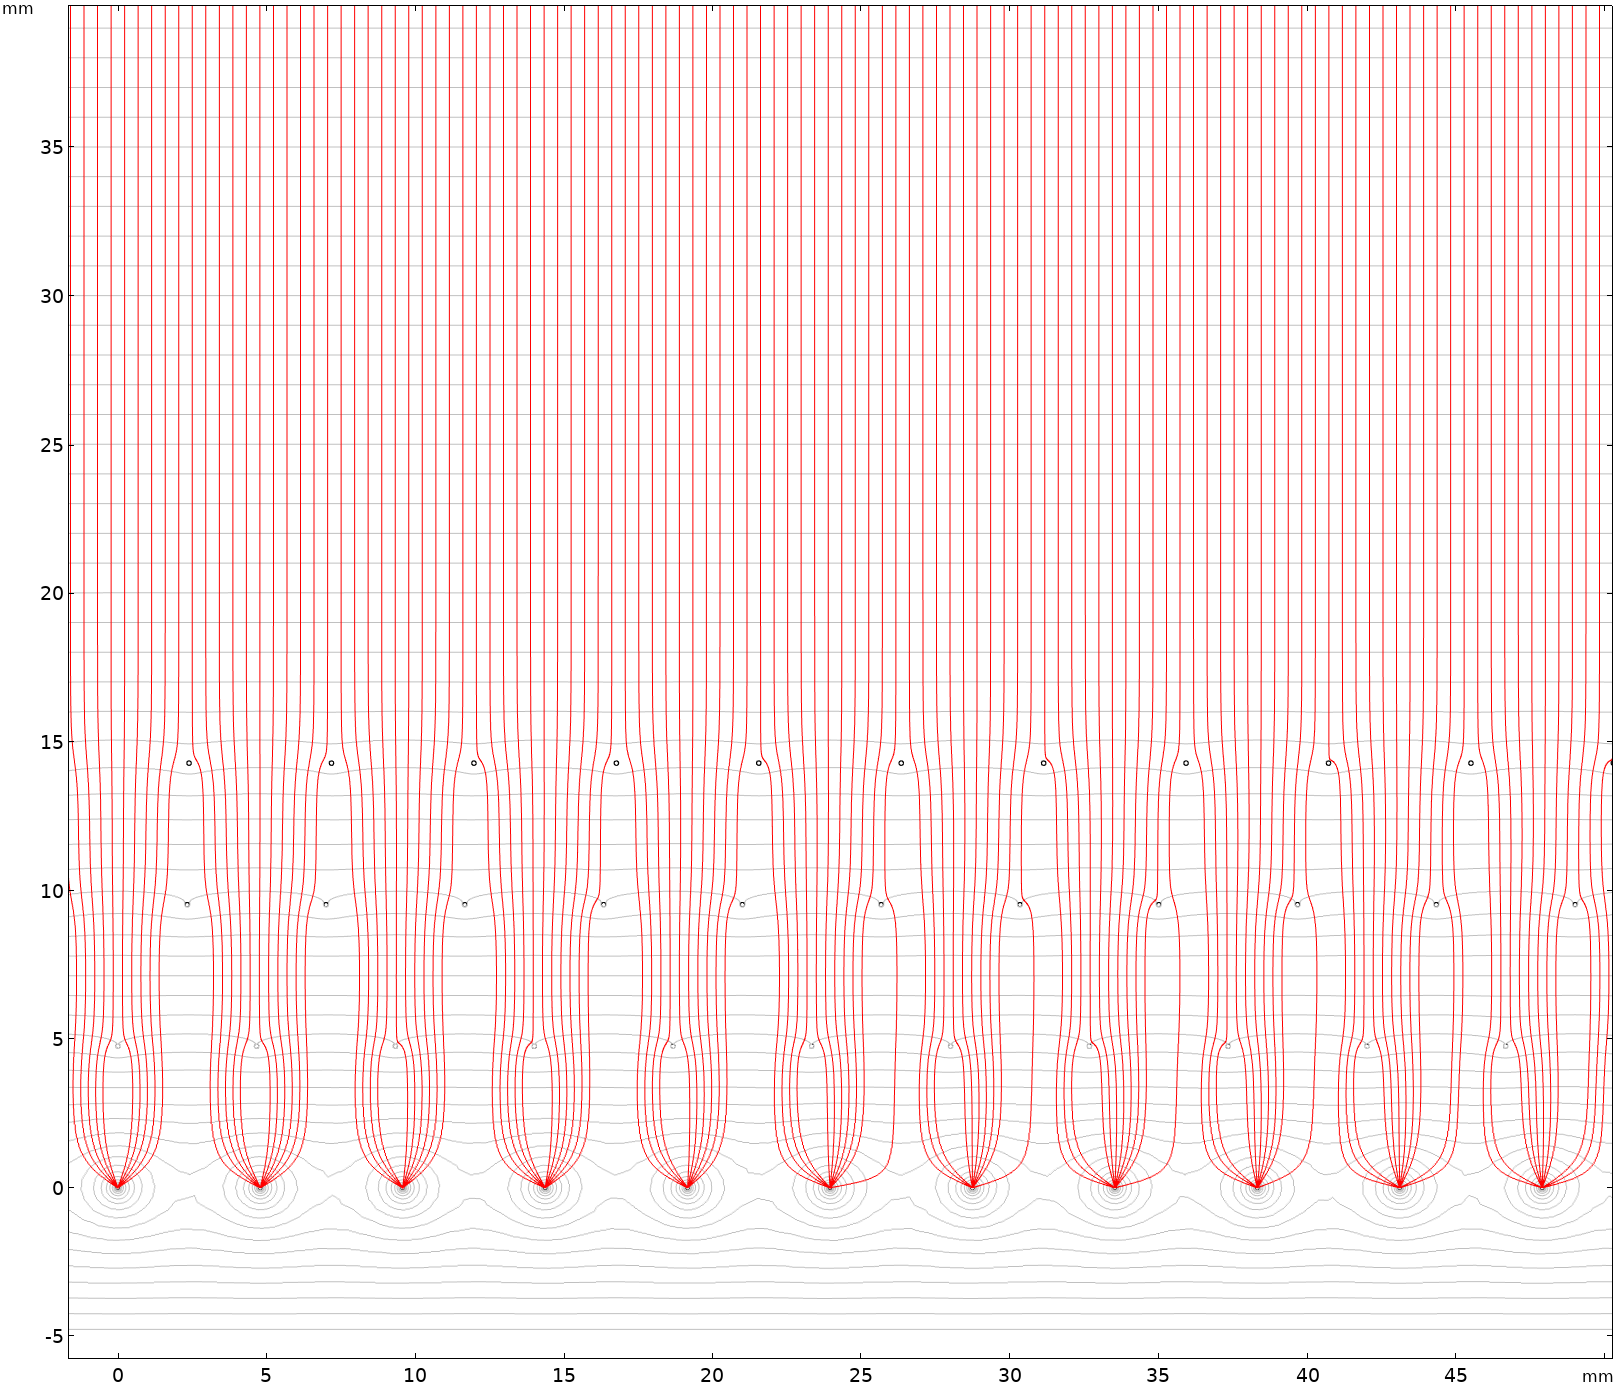
\includegraphics[width=0.42\textwidth]{graphics/sp-apa-field-lines-2D.png}
b) 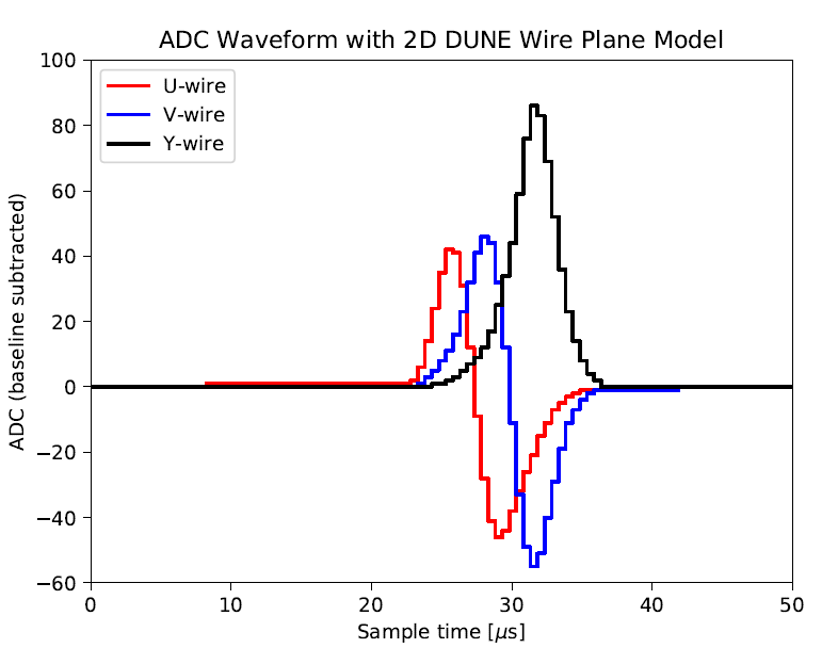
\includegraphics[width=0.5\textwidth]{graphics/sp-apa-ADC-waveform.png}
\end{dunefigure}


\item \textbf{Wire type and tension:}  The wire selected for the \dword{apa}s is \SI{152}{$\mu$m} beryllium (\num{1.9}\%) copper wire, %\footnote{\url{http://www.lfa-wire.com/heat-treatable-alloy-25_c17200-and-c17300.htm}}
chosen for its mechanical and electrical properties, ease of soldering, and cost.  The tension on the wires, combined with intermediate support combs on the \dword{apa} frame cross beams (described in Section~\ref{sec:combs}), ensure that the wires are held taut in place with minimal sag.  Wire sag can affect the precision of reconstruction, as well as the transparency of the \dword{tpc} wire planes.  The tension must be low enough that when the wires are cooled, which increases their tension due to thermal contraction, they stay safely below the break load of the beryllium copper wire.  A tension of $6\pm$\SI{1}{N} is the baseline for \dword{dune}, to be confirmed after \dword{pdsp} analysis is completed.  %To further mitigate wire slippage and its effect on detector performance, each wire in the \dword{apa} is anchored twice at all end points with both solder and epoxy.  
See Section~\ref{sec:fdsp-apa-wires} for more details about the \dword{apa} wires.

\end{itemize}

Table~\ref{tab:apaparameters} summarizes some of the principal design parameters for the \dword{spmod} 
\dwords{apa}.

\begin{dunetable}[APA design parameters]{lr}{tab:apaparameters}
{\dword{apa} design parameters}   
Parameter & Value  \\ \toprowrule
Active height & \SI{5.984}{m} \\ \colhline
Active width & \SI{2.300}{m} \\ \colhline
Wire pitch ($U,V$) & \uvpitch \\ \colhline
Wire pitch ($X,G$) & \xgpitch \\ \colhline
Wire pitch tolerance & \wirepitchtol \\ \colhline
Wire plane spacing & \planespace \\ \colhline
Wire plane spacing tolerance & $\pm$\SI{0.5}{mm} \\ \colhline
Wire Angle (w.r.t. vertical) ($U,V$) & \apainducwireangle{} \\ \colhline
Wire Angle (w.r.t. vertical) ($X,G$) & \apacollwireangle \\ \colhline
Number of wires / \dword{apa} & 960 ($X$), 960 ($G$), 800 ($U$), 800 ($V$) \\ \colhline
Number of electronic channels / \dword{apa} & 2560 \\ \colhline
%Wire Tension & \SI{5.0}{N} \\ \colhline
%Wire Tension Tolerance & $\pm$\SI{1}{N} \\ \colhline
Wire material & beryllium copper \\ \colhline
Wire diameter & 152 $\mu$m \\ 
%Wire Resistivity & 7.68 $\mu\Omega$-cm $@$ 20$^{\circ}$ C \\ \colhline
%Wire Resistance/m & 4.4 $\Omega$/m $@$ 20$^{\circ}$ C \\ \colhline
%Frame Planarity & 5 mm \\ \colhline
%Photon Detector Slots & 10 \\
\end{dunetable}


%%%%%%%%%%%%%%%%%%%%%%%%%%%%%%%%%%%%%%%%%%%%%%%%%%%%%%%%%%%%%%%%%%%%%%
\subsection{Support Frames}
\label{sec:fdsp-apa-frames}

The \dword{apa} frames are built of rectangular hollow section (RHS) stainless steel tubes.  Figure~\ref{fig:apa-frame-full} shows three long tubes, a foot tube, a head tube, and eight cross-piece ribs that bolt together to create the \SI{6.0}{m} tall by \SI{2.3}{m} wide frame. All hollow sections are \SI{10.2}{cm} (\SI{4}{in}) deep with varying widths depending on their role. 

\begin{dunefigure}[Bare APA frame drawing]{fig:apa-frame-full}
{A \dword{dune} \dword{apa} frame showing the \num{13} separate stainless steel tube sections that bolt together to form a complete frame.  The long tubes and foot tube are a \num{10.2}$\times$\SI{10.2}{cm} (\num{4}$\times$\SI{4}{inch}) cross section, the head tube is \num{10.2}$\times$\SI{15.2}{cm} (\num{4}$\times$\SI{6}{inch}), and the ribs are \num{10.2}$\times$\SI{5.1}{cm} (\num{4}$\times$\SI{2}{inch}). 
}
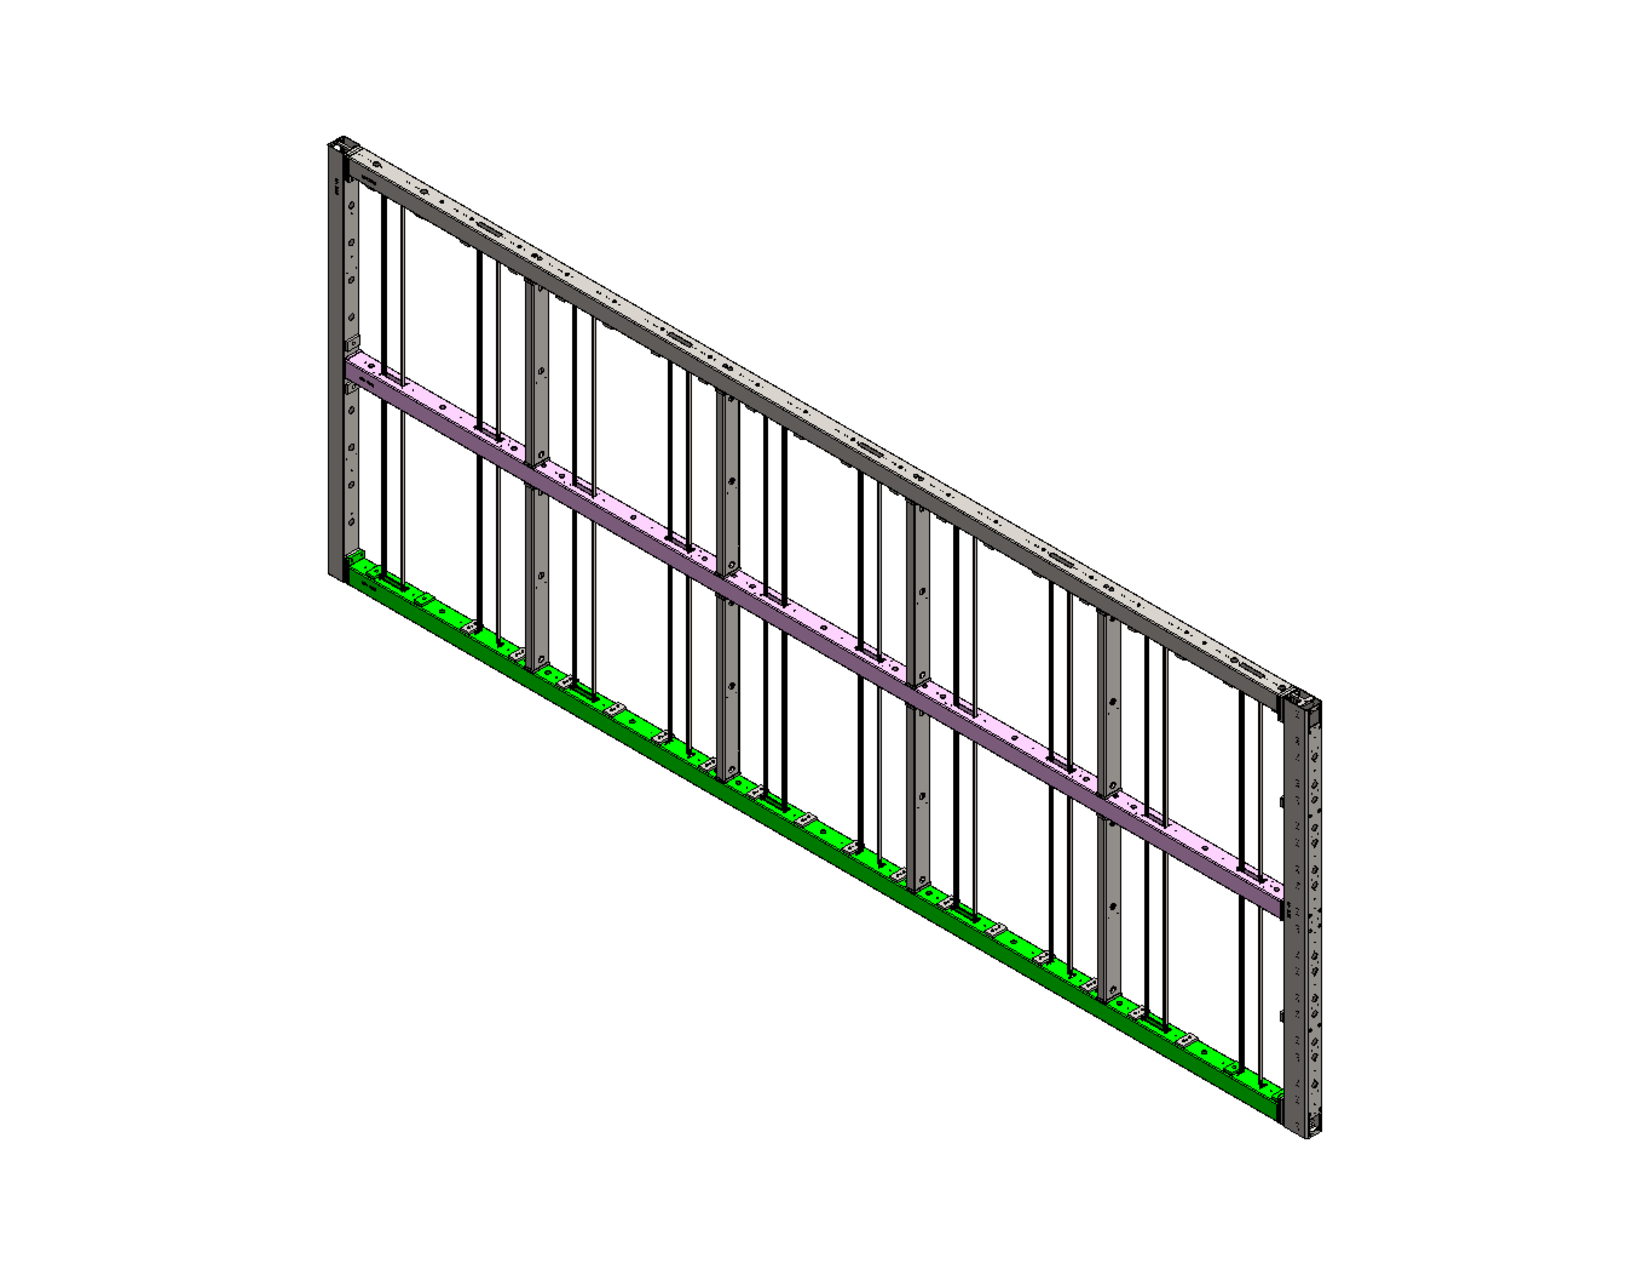
\includegraphics[width=1\textwidth]{sp-apa-frame-full-2.pdf}
\end{dunefigure}

\begin{dunefigure}[APA frame construction  details]{fig:apa-frame-details}
{\dword{apa} frame construction details. Top: The corner joint between the foot tube and the side tube. Middle: The joint between the side tube and a rib. Bottom: The joint between the head tube and the side tube.}

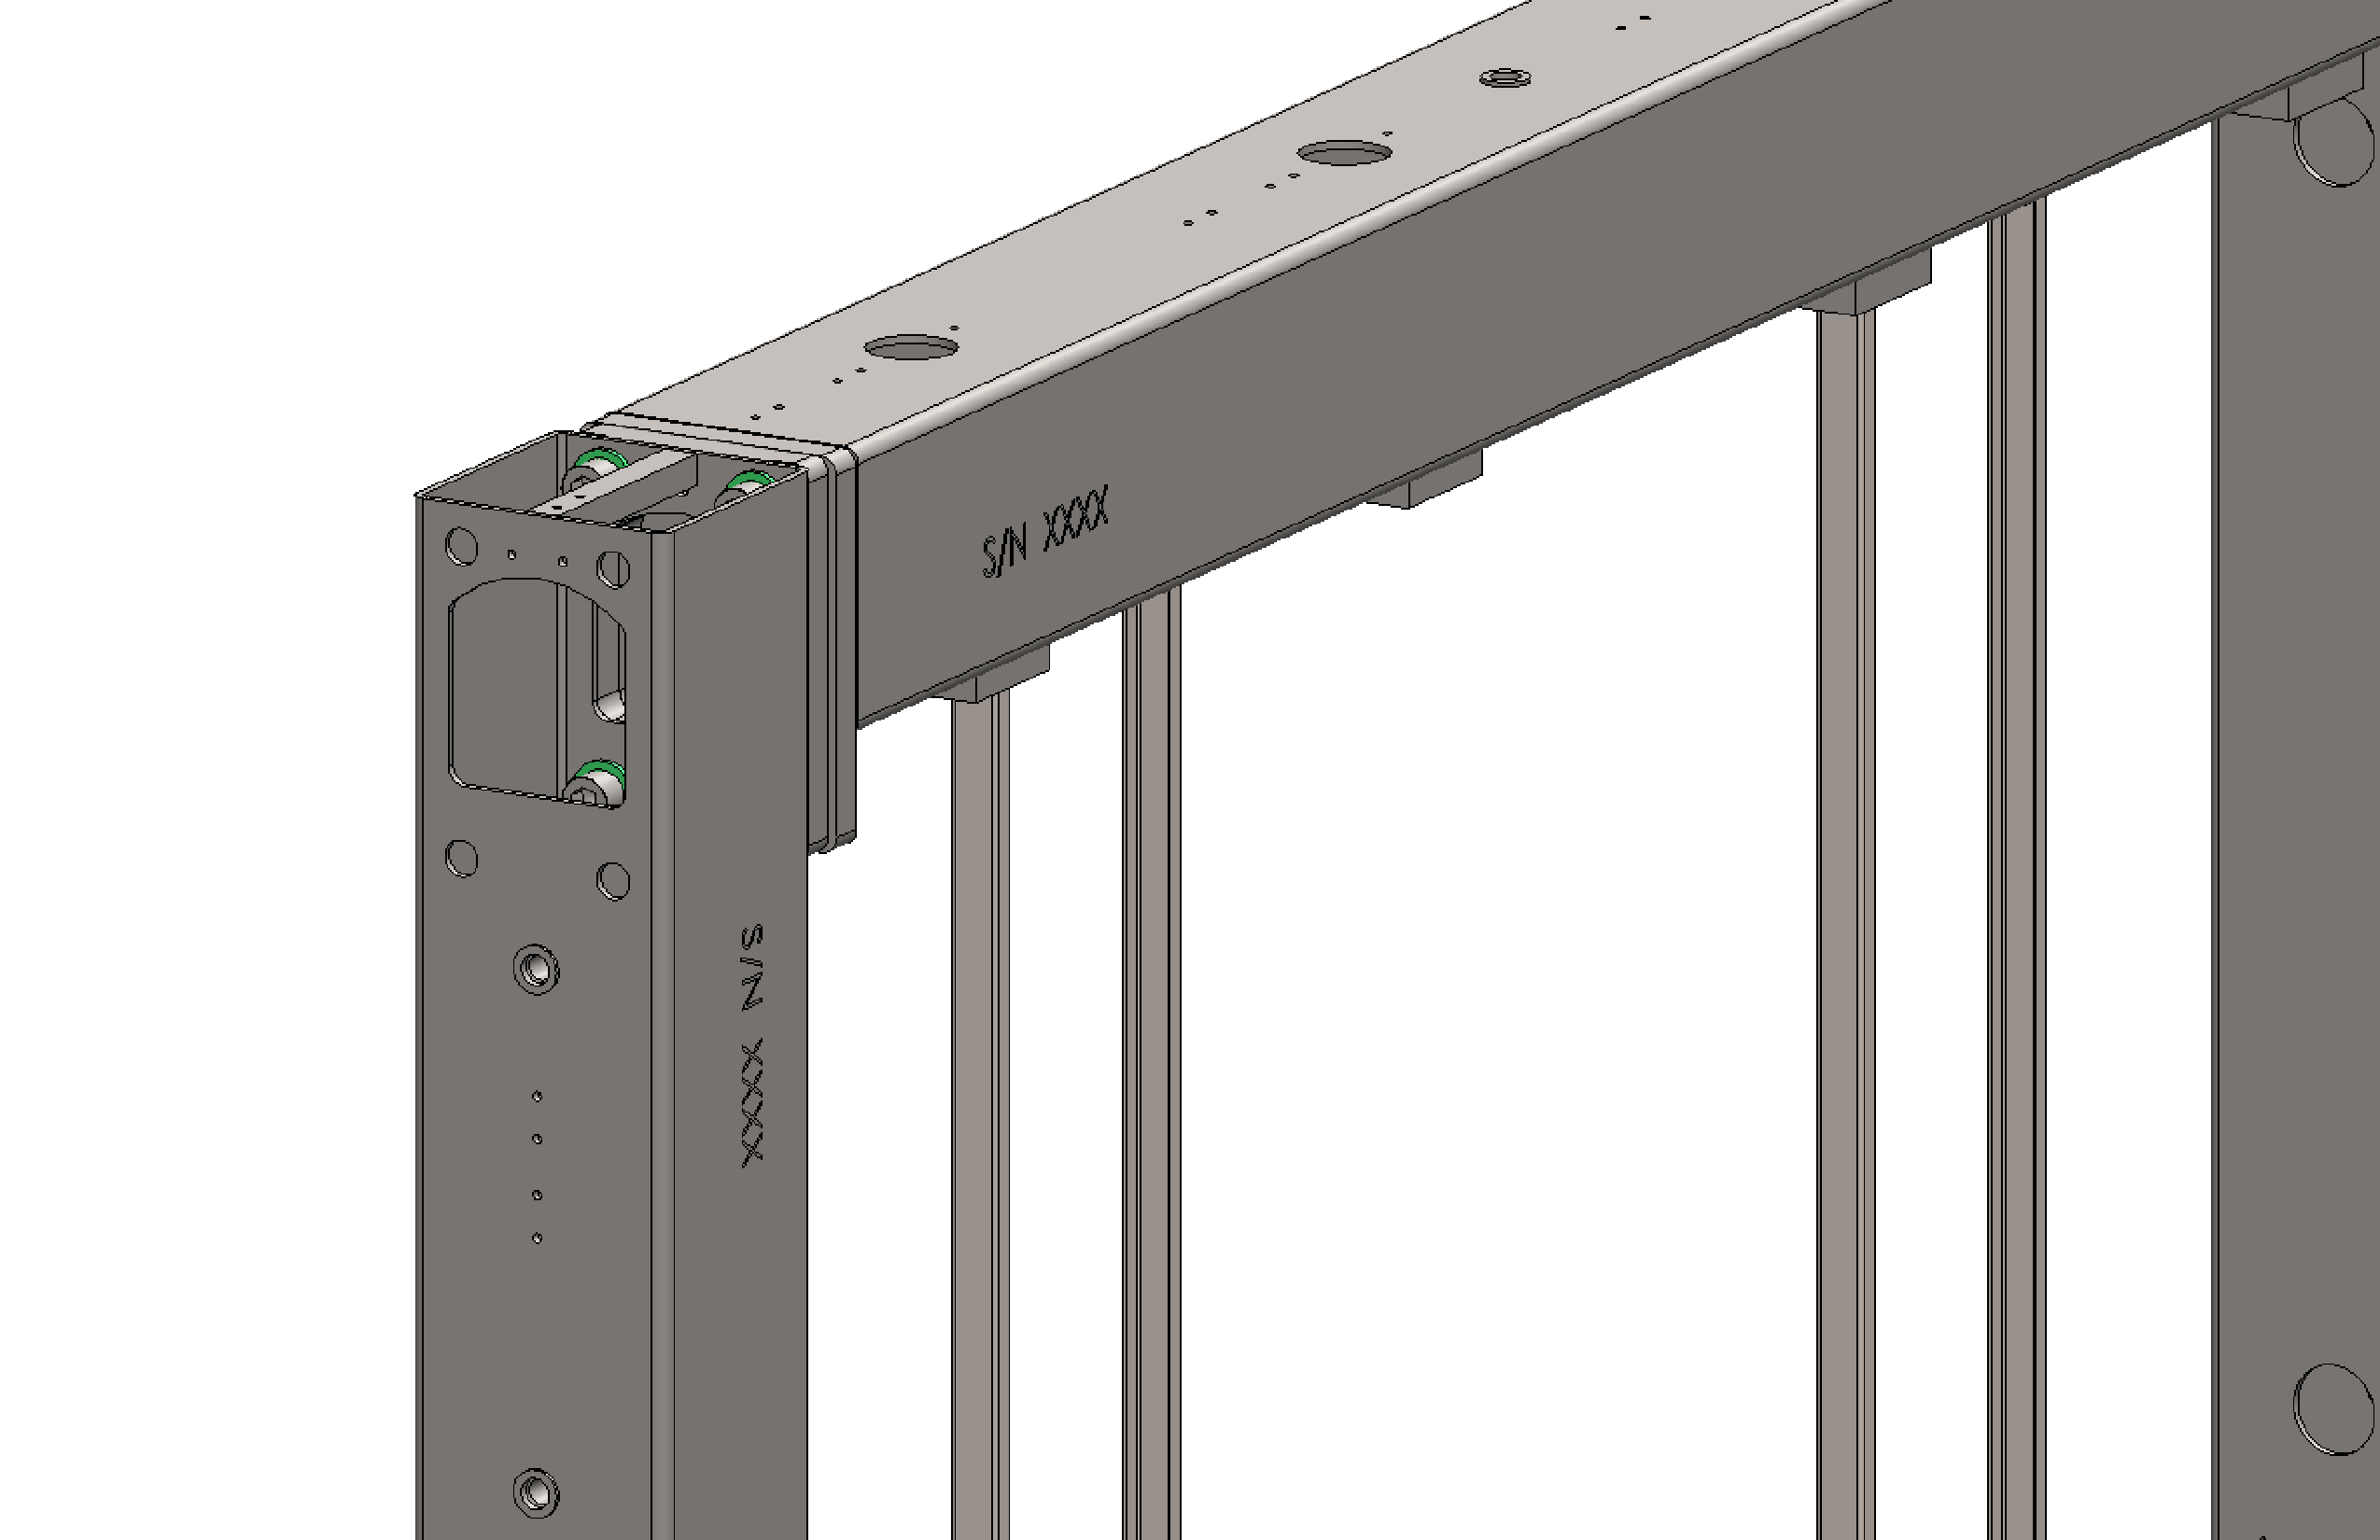
\includegraphics[height=0.31\textheight,trim=0mm 0mm 0mm 0mm,clip]{sp-apa-frame-foot.pdf}
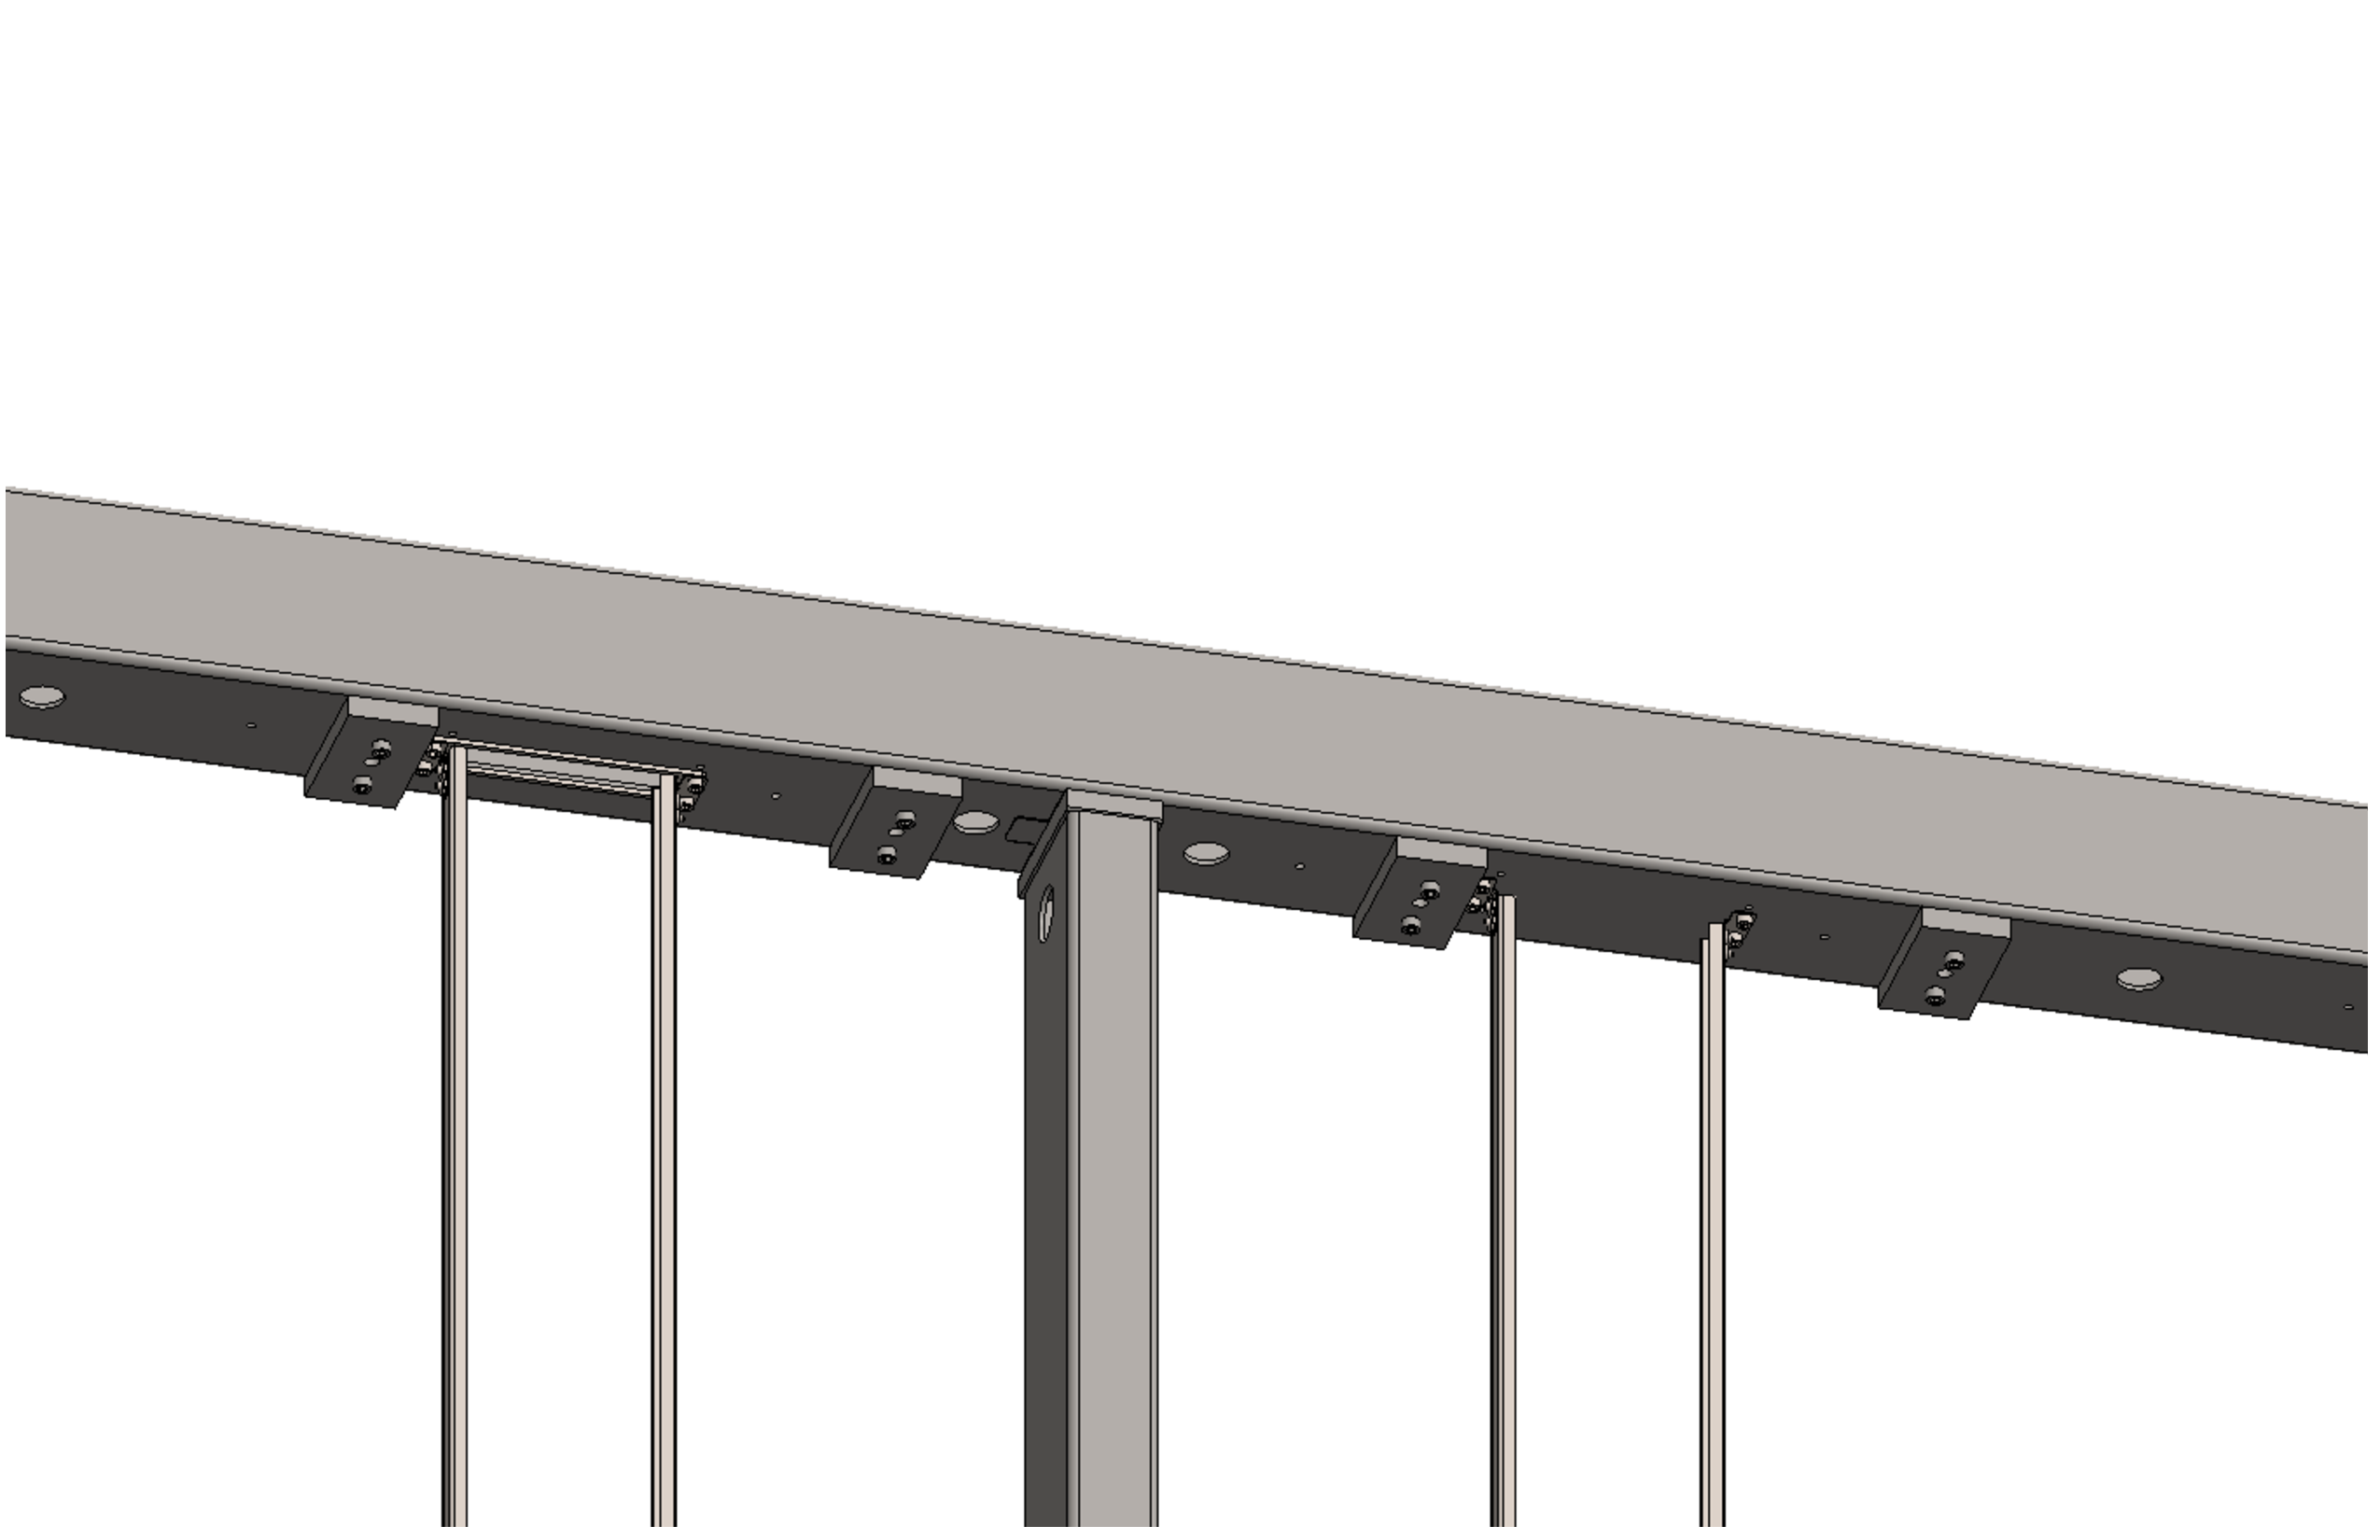
\includegraphics[height=0.28\textheight,trim=0mm 0mm 0mm 0mm,clip]{sp-apa-frame-side-joint.pdf}
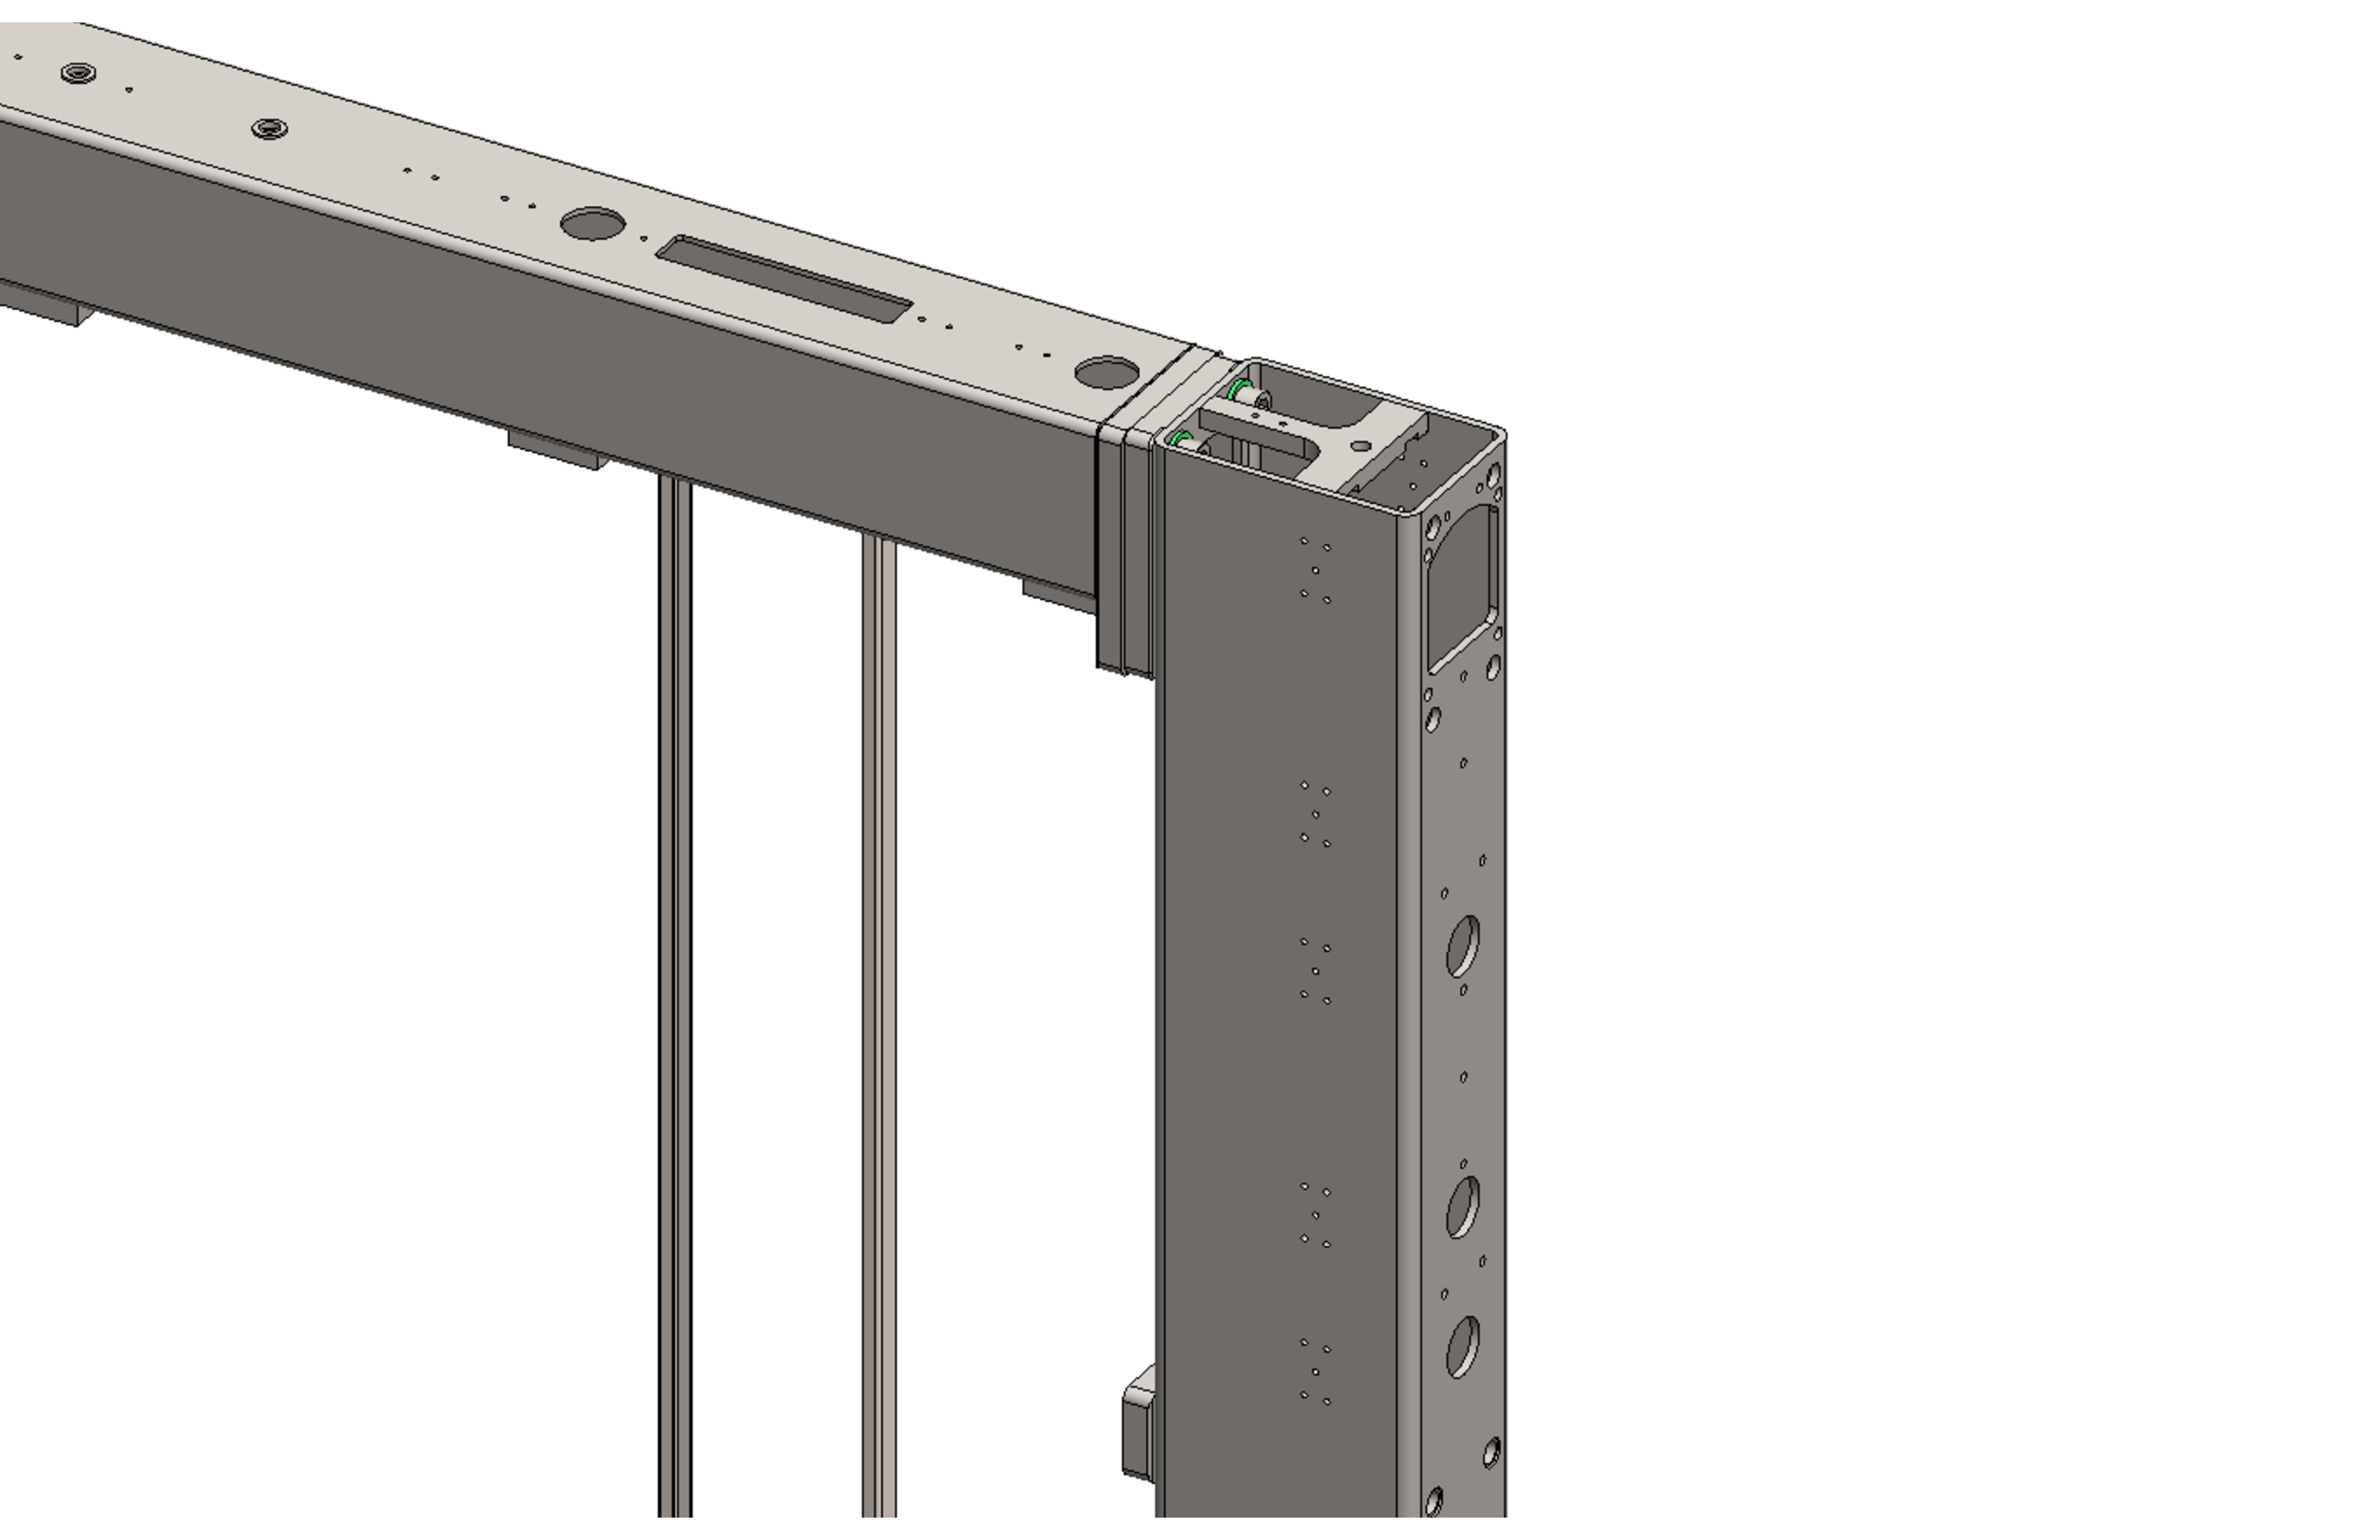
\includegraphics[height=0.32\textheight]{sp-apa-frame-head.pdf}
\end{dunefigure}

The head and foot tubes are bolted to the side and center pieces via abutment flanges welded to the tubes. In production, the pieces can be individually machined to help achieve the flatness and shape tolerances.  During final assembly, shims are used to create a flat, rectangular frame of the specified dimensions.  The central cross pieces are similarly attached to the side pieces.  Figure~\ref{fig:apa-frame-details} shows models of the different joints.   



The \dword{apa} frames also house the \dword{pds} (Chapter~\ref{ch:fdsp-pd}).  %In the \dword{pdsp} design, 
Rectangular slots are machined in the outer frame tubes and guide rails are used to slide in \dword{pd} elements from the edges. %although alternative \dword{pd} designs are being considered for the \dwords{spmod}. %DUNE. 
(See Section~\ref{sec:fdsp-apa-intfc} for more details on interfacing with the \dword{pds}.)   

In a \dword{fd} \dword{spmod}, pairs of \dword{apa} frames will be mechanically connected to form a \tpcheight %\SI{12}{m} 
tall structure with electronics for \dword{tpc} readout at both the top and bottom of this two-frame assembly and \dwords{pd} installed throughout.  The \dword{apa} frame design, therefore, must support cable routing to the top of the detector from both the bottom \dword{apa} readout electronics and the \dwords{pd} mounted throughout both \dword{apa}s.  Section~\ref{sec:fdsp-apa-intfc} discusses the interfaces.



%%%%%%%%%%%%%%%%%%%%%%%%%%%%%%%%%%%%%%%%%%%%%%%%%%%%%%%%%%%%%%%%%%%%%
\subsection{Grounding Mesh}
\label{sec:fdsp-apa-mesh}

Beneath the layers of sense wires, the conducting surface should be uniform to evenly terminate the \efield and improve the uniformity of field lines around the wire planes. A fine woven mesh that is \num{85}\% optically transparent is used to allow scintillation photons to pass through to the \dwords{pd} mounted inside the frame.  The mesh also shields the \dword{apa} wires from spurious electrical signals from other parts of the \dword{apa} or the \dword{pd} system.  

In the \dword{pdsp} \dword{apa}s, the mesh was installed in four long sheets, along the length of the left- and right-hand halves of each side of the \dword{apa} and epoxied directly to the frame. This approach to mesh installation was found to be slow and cumbersome.  For the \dword{dune} mass production, a modular window-frame design is being developed, where mesh is pre-stretched over smaller sub-frames that can be clipped into each gap between cross beams in the full \dword{apa} frame.   This improves the reliability of the installed mesh (more uniform tension across the mesh) and allows much easier installation on the \dword{apa} frame. The mesh will be woven of conducting 304 stainless steel \SI{89}{\um} wire. It will be mounted on 304 stainless steel \SI{20}{mm}$\times$\SI{10}{mm} box section frames,  stretched over the frame with jigs and pneumatic actuators built for the purpose, and TIG welded around the top surface and again around the side surfaces. Five different panel designs are needed to match the openings in the \dword{apa} frames: two for the foot end, two for the head end, and one for the central panels that are all the same. There are 20 panels per \dword{apa}. Stainless steel brackets will be fixed to the inner window sections of the \dword{apa} frame and the panels will be secured into position using steel fasteners. The design ensures good electrical contact between the mesh and the frame. A full-scale \dword{apa} (\dword{apa}-07) has been built at Daresbury Lab for \dword{ce} testing at \dword{cern} using the mesh panel design. Figure~\ref{fig:tpc-apa-mesh} shows images of the mesh design and the prototypes built for \dword{apa} 7.

\begin{dunefigure}[Photos of APA grounding mesh]{fig:tpc-apa-mesh}
{\dword{apa} grounding mesh construction and installation. a) The mesh panel stretching jig, b) mesh being welded to the support frame, c) model showing the mesh sub-frame (in dark gray) fitting into the \dword{apa} frame (green), and d) photo of an installed mesh panel in \dword{apa} 7.}
\mbox{a) 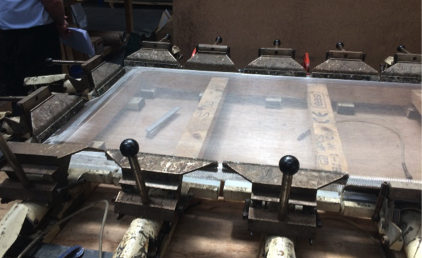
\includegraphics[height=0.23\textheight]{sp-apa-mesh-jig.png} \hspace{0.0mm}
b) 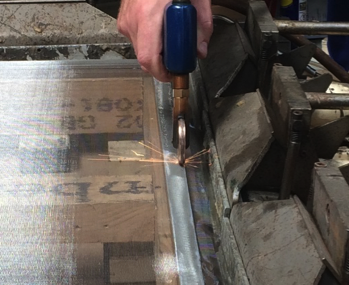
\includegraphics[height=0.23\textheight]{sp-apa-mesh-weld.png}} \\
\vspace{3mm}
\hspace{0.4mm}
\mbox{c) 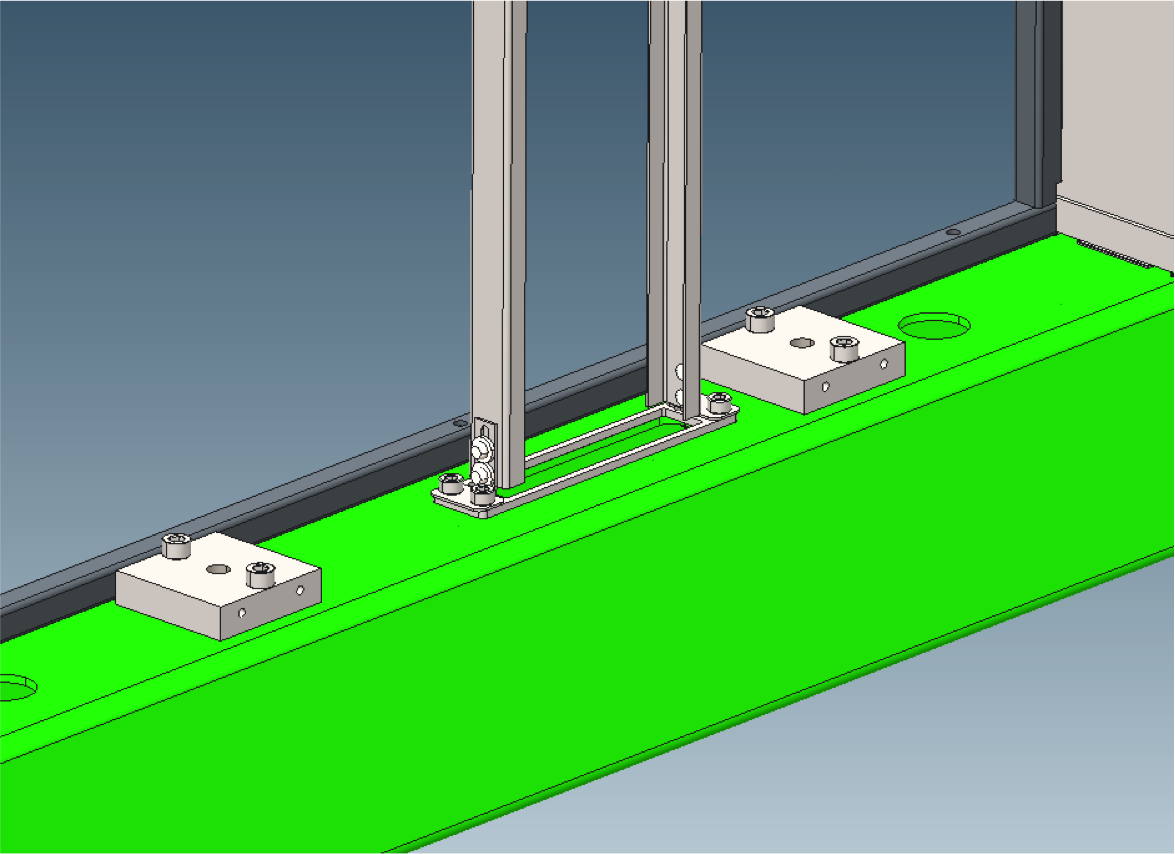
\includegraphics[height=0.23\textheight]{sp-apa-mesh-install-design.png}
d) 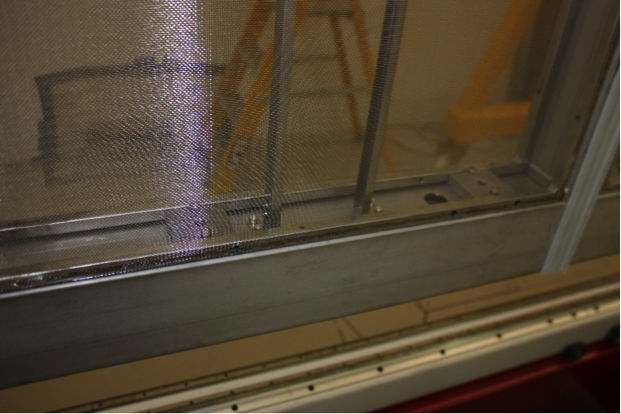
\includegraphics[height=0.23\textheight]{sp-apa-mesh-installed.png}}
\end{dunefigure}




%%%%%%%%%%%%%%%%%%%%%%%%%%%%%%%%%%%%%%%%%%%%%%%%%%%%%%%%
\subsection{Wires}
\label{sec:fdsp-apa-wires}

The \SI{152}{$\mu$m} (\SI{.006}{in}) diameter beryllium copper (CuBe) wire chosen for use in the \dword{apa}s is known for its high durability and yield strength. It is composed of \num{98}\,\% copper, \num{1.9}\,\% beryllium, and a negligible amount of other elements. Each \dword{apa} contains a total of \SI{23.4}{km} of wire.  

The key properties for its use in the \dword{apa}s are low resistivity, high tensile or yield strength, and a coefficient of thermal expansion suitable for use with the \dword{apa}'s stainless steel frame (see Table~\ref{tab:wire} for a summary of properties).  Tensile strength of the wire describes the wire-breaking stress.  The yield strength is the stress at which the wire starts to take a permanent (inelastic) deformation and is the important limit for this case. The wire spools purchased from Little Falls Alloys\footnote{Little Falls Alloys\texttrademark, \url{http://www.lfa-wire.com/}} for use on \dword{pdsp} were measured to have tensile strength higher than \SI{1380}{MPa} and yield strength more than \SI{1100}{MPa} (\SI{19.4}{N} for \SI{152}{$\mu$m} diameter wire).  The stress while in use is approximately \SI{336}{MPa} (\SI{6}{N}), leaving a comfortable margin.

The \dword{cte} describes how a material expands or contracts with changes in temperature.  The \dwords{cte} of CuBe alloy and \num{304} stainless steel are very similar.  Integrated down to \SI{87}{K}, they are \SI{2.7}{mm/m} for stainless steel and \SI{2.9}{mm/m} for CuBe. The wire contracts slightly more than the frame, so for a wire starting at \SI{6}{N} at room temperature the tension increases to around \SI{6.5}{N} when everything reaches \lar temperature.  

The rate of change in wire tension during \cooldown is also important.  In the worst case, the wire cools quickly to \SI{87}{K} before any significant cooling of the much larger frame.  In the limiting case with complete contraction of the wire and none in the frame, the tension would peak around \SI{11.7}{N}, which is still well under the \SI{19}{N} yield tension. In practice, however, the cooling will be done gradually to avoid this tension spike as well as other thermal shocks to the detectors.

\begin{dunetable}[Beryllium copper (CuBe) wire properties]{lr}{tab:wire}{Summary of properties of the beryllium copper wire used on the \dword{apa}s.}
Parameter & Value \\ \toprowrule
Resistivity & 7.68 $\mu\Omega$-cm $@$ 20$^{\circ}$ C \\ \colhline
Resistance & 4.4 $\Omega$/m $@$ 20$^{\circ}$ C \\ \colhline
Tensile strength (from property sheets)  & \SI{1436}{MPa} / \SI{25.8}{N} for \SI{152}{$\mu$m} wire \\ \colhline
%Tensile strength (from actual wire)  & \SI{212530}{psi} / \SI{26.4}{N} for \SI{152}{$\mu$m} wire \\ \colhline
CTE of beryllium copper integrated to \SI{87}{K}  & \SI{2.9e-3}{m/m} \\ \colhline
CTE of stainless steel integrated to \SI{87}{K}  & \SI{2.7e-3}{m/m} \\
\end{dunetable}


%%%%%%%%%%%%%%%%%%%%%%%%%%%%%%%%%%%%%%%%%%%%%%%%%%%%%%%%%%%%%%%%
\subsection{Wire Boards and Anchoring Elements}
\label{sec:fdsp-apa-boards}

To guide and secure the \num{3520} wires on an \dword{apa}, stacks of custom \frfour circuit boards attach all along the outside edges of the frame, as shown in the engineering drawings in Figure~\ref{fig:apa-wire-boards}.  There are \num{337} total circuit boards on each \dword{apa} (\num{50550} in an \dword{spmod} with \num{150} \dword{apa}s), where this number includes 204 wire boards ($X/V/U/G = 30/72/72/30$), 72 cover boards to protect the wire solder pads and traces on the top layer of wire boards, 20 capacitive-resistance (\dword{cr}) boards, 20 adapter boards to connect the \dword{cr}s to the \dword{ce}, 20 $G$-layer bias boards, and one \dword{shv} board to distribute bias voltages to the planes.  Figure~\ref{fig:sp-apa-head-xsec} shows the positions of the boards at the head of the \dword{apa} and the path connecting \dword{tpc} wires to the \dword{ce}.  %Below, the wire boards and \dword{cr} boards are described in more detail.

\begin{dunefigure}[Wire carrier board layout on the APA frames]{fig:apa-wire-boards}
{Engineering drawings that illustrate the layering of the wire carrier boards that are secured along the perimeter of the \dword{apa} steel frames. Left: The full set of $V$-layer boards.  Right: Detail showing the stack of four boards at the head end of the \dword{apa} (bottom to top: $X,V,U,G$).}
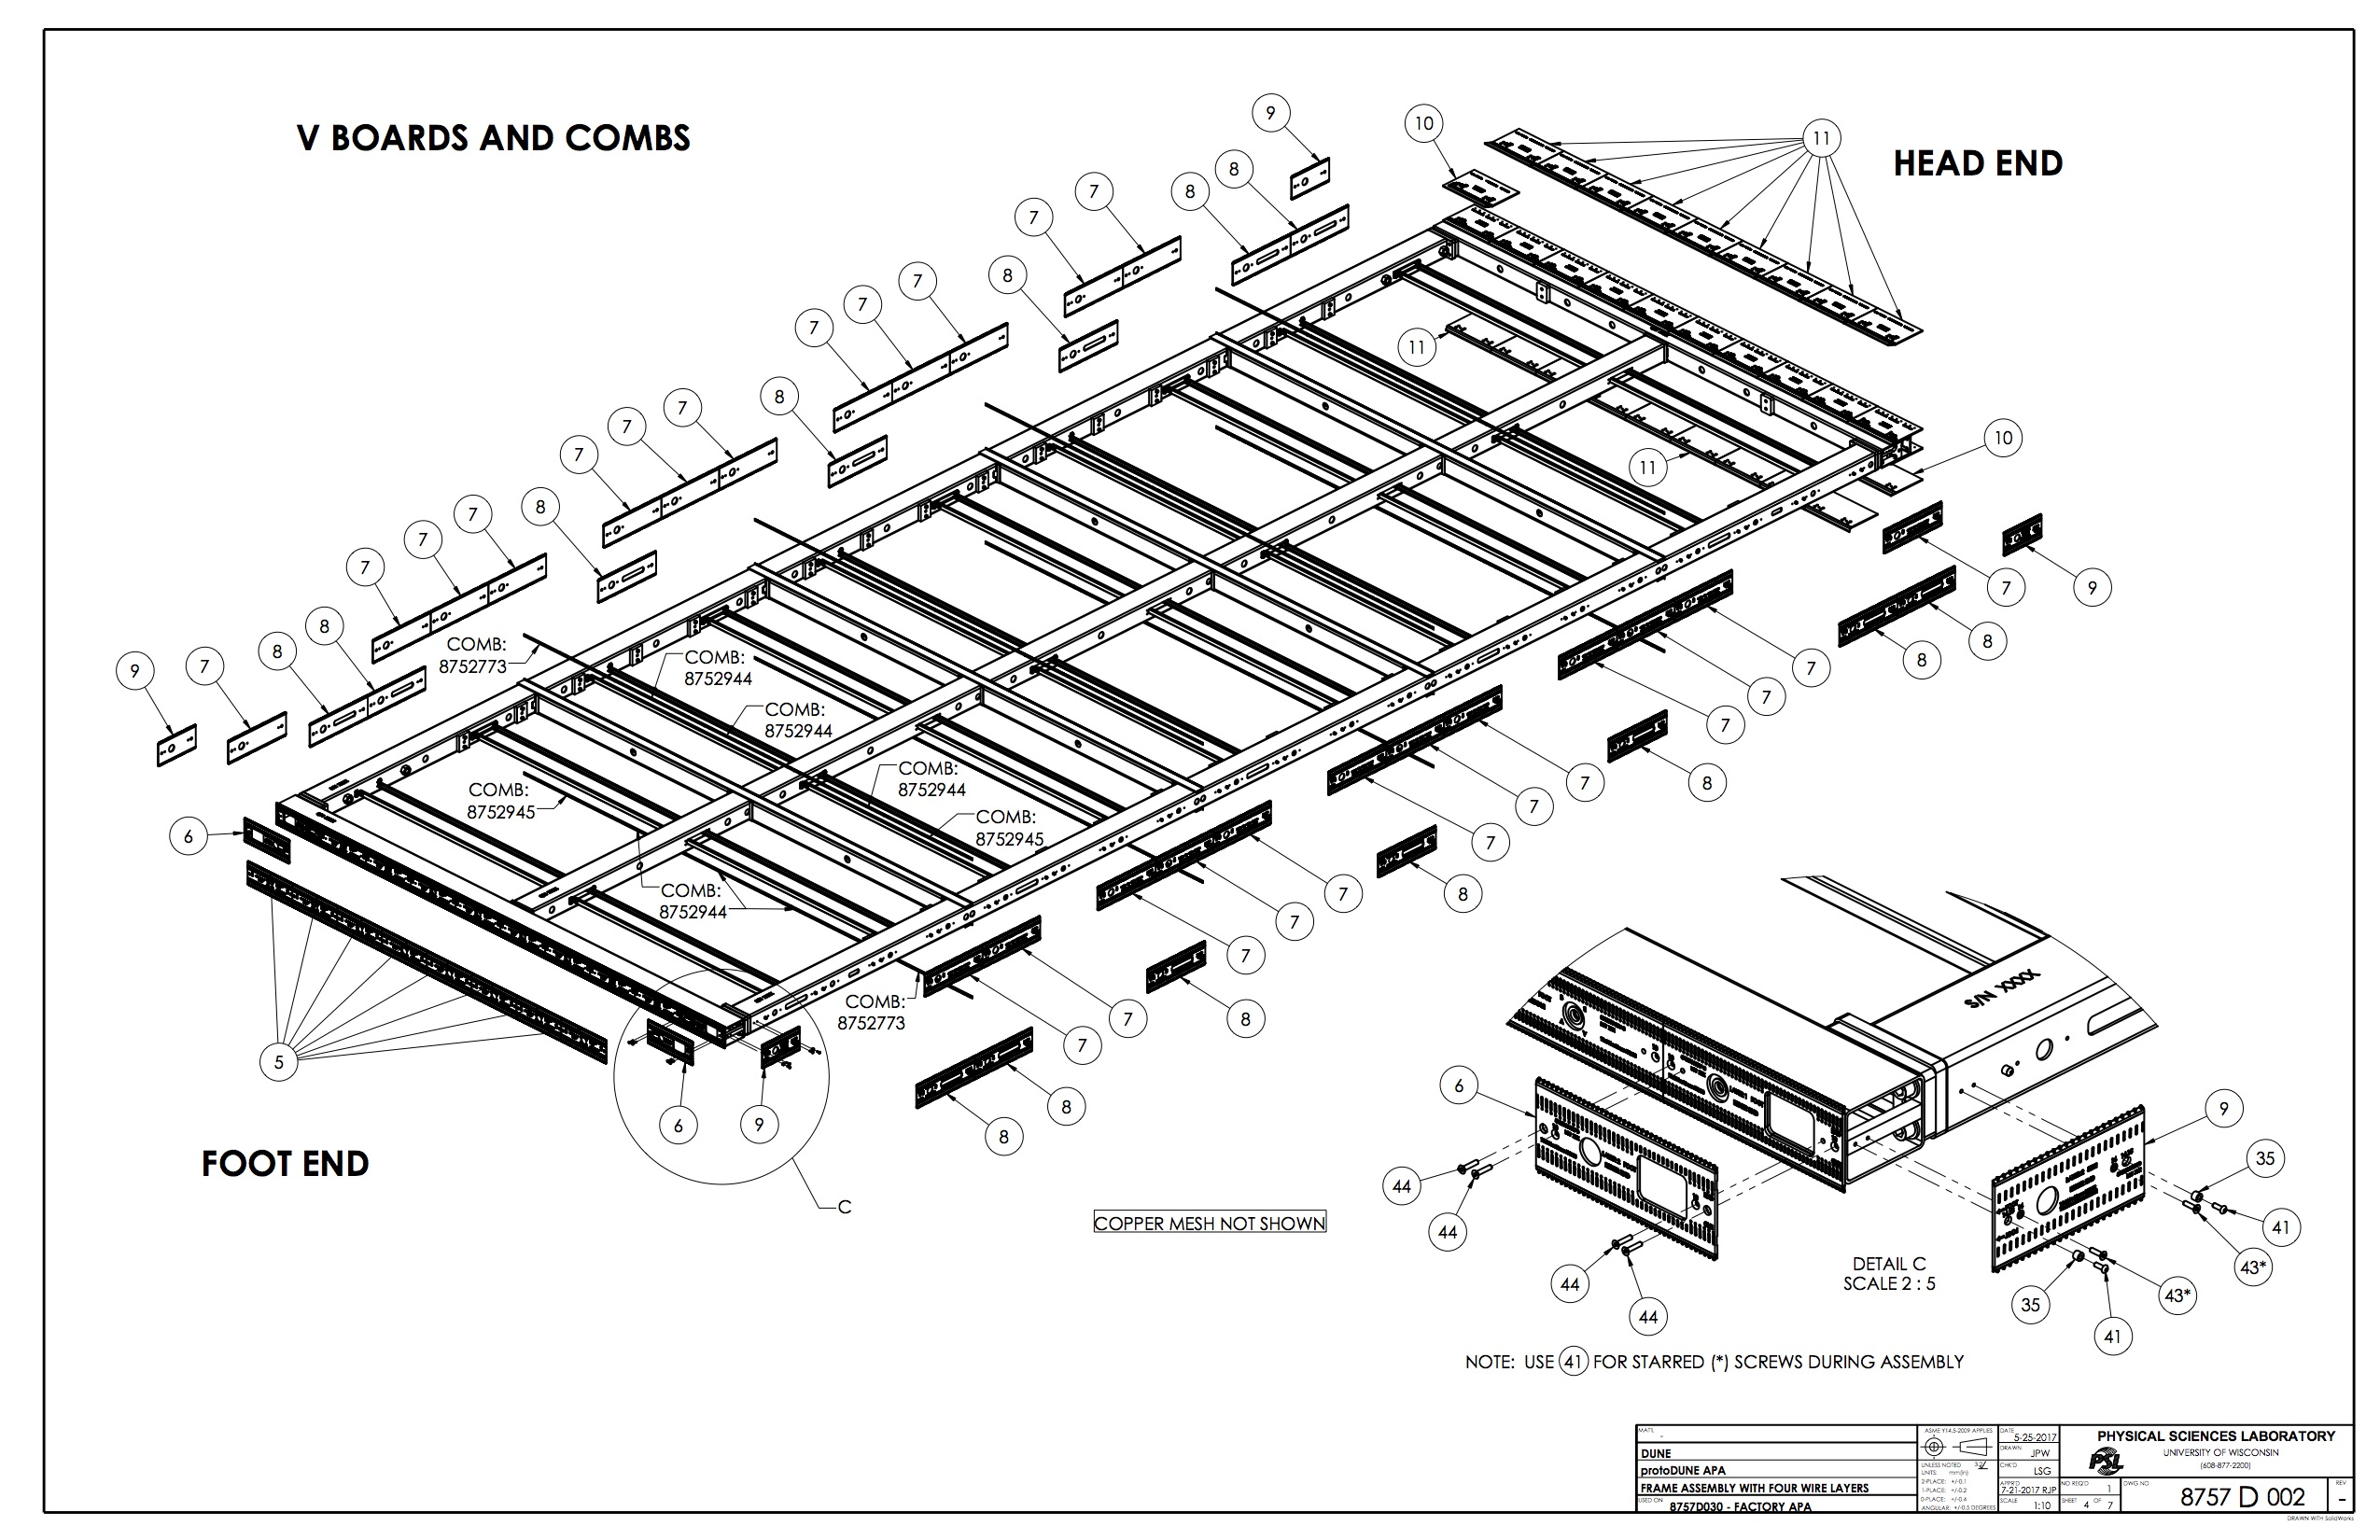
\includegraphics[width=0.48\textwidth,trim = 12mm 0mm 5mm 0mm,clip]{sp-apa-drawing-v-boards-exploded.jpg}
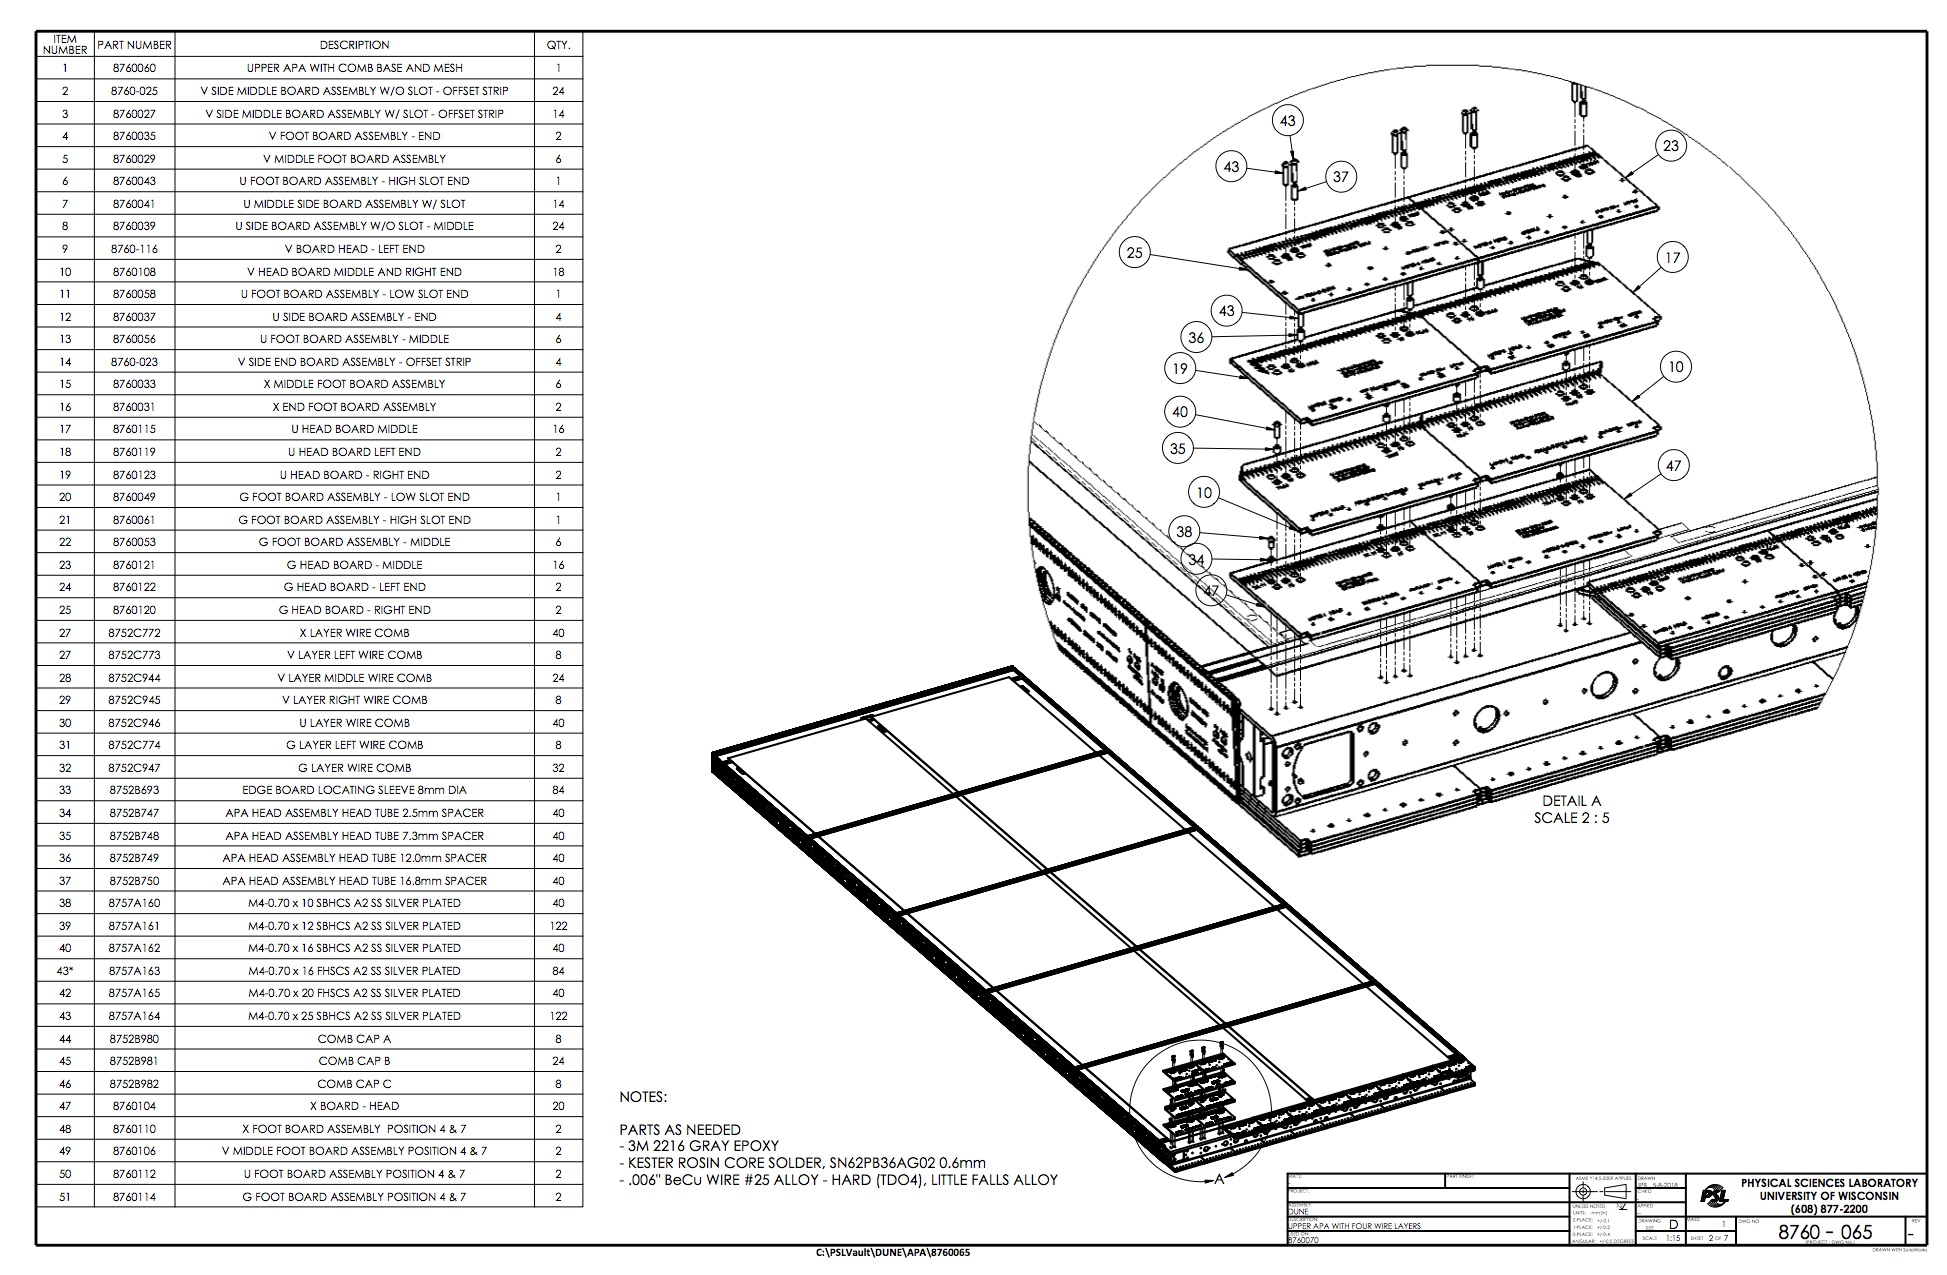
\includegraphics[width=0.48\textwidth,trim = 12mm 0mm 5mm 0mm,clip]{sp-apa-drawing-board-stack-detail.jpg}
\end{dunefigure}


%%%%%%%%%%%%%%%%%%%%%%%%%%%%%%%%%%%%%%%
\subsubsection{Head Wire Boards}
\label{sec:fdsp-apa-headboards}

All \dword{apa} wires terminate on wire boards stacked along the electronics end of the \dword{apa} frame.  The board stack at the head end is shown in an engineering drawing in the right panel of Figure~\ref{fig:apa-wire-boards}. A photograph showing the head boards and $G$-bias boards on one of the completed \dword{pdsp} \dword{apa}s is shown in Figure~\ref{fig:tpc_apa_electronics_connectiondiagram}. Attaching the wire boards begins with the $X$-plane (innermost). Once the $X$-plane wires are strung on both sides of the \dword{apa} frame, they are soldered and epoxied to their wire boards and trimmed. Next, the $V$-plane boards are epoxied in place and the $V$ wires installed, followed by the $U$-plane boards and wires, and finally the $G$-plane boards and wires. The wire plane spacing of \planespace %\SI{4.75}{mm} 
is set by the thickness of these wire boards.   

\begin{dunefigure}[Wire board stack at the head end of an \dshort{apa}]{fig:tpc_apa_electronics_connectiondiagram}{The wire board stack at the head end of an \dword{apa}. The four wire boards within a stack can be seen on both the top and bottom sides of the \dword{apa}.  Also visible are the T-shaped brackets that will hold the \dword{ce} boxes when electronics are installed.   
}
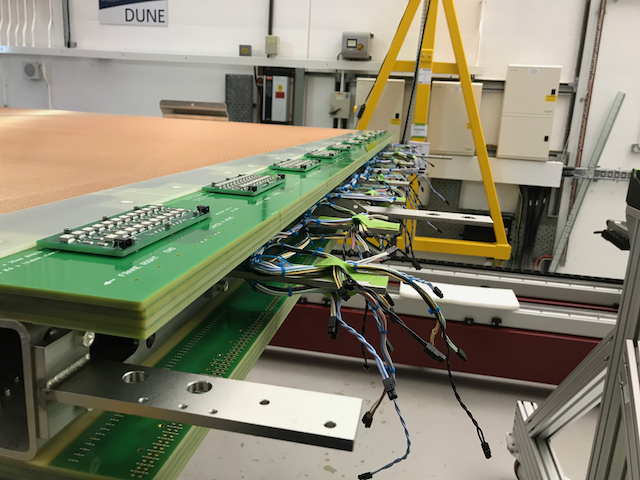
\includegraphics[width=0.6\textwidth, trim=0mm 0mm 0mm 15mm, clip]{sp-apa-board-stack.png}
\end{dunefigure} 

Mill-Max\footnote{Mill-Max\texttrademark{}, \url{https://www.mill-max.com/}} pins and sockets provide electrical connections between circuit boards within a stack. They are pressed into the circuit boards and are not repairable if damaged. To minimize the possibility of damaged pins, the boards are designed so that the first wire board attached to the frame has only sockets. All boards attached subsequently contain pins that plug into previously mounted boards. This process eliminates exposure of any pins to possible damage during winding, soldering, or trimming.

The $X$, $U$ and $V$ layers of wires are connected to the \dword{ce} (housed in boxes mounted on the \dword{apa}) either directly ($V$) or through DC-blocking capacitors ($U,X$).  Ten stacks of wire boards are installed across the width of each side along the head of the \dword{apa}.  The $X$-layer board in each stack has room for \num{48} wires, the $V$-layer has 40 wires, the $U$-layer \num{40} wires, and the $G$-layer \num{48} wires.  Each board stack, therefore, has \num{176} wires but only \num{128} signal channels since the $G$ wires are not read out. With a total of \num{20} stacks per \dword{apa}, this results in \num{2560} signal channels per \dword{apa} and a total of \num{3520} wires starting at the top of the \dword{apa} and ending at the bottom. Many of the capacitors and resistors that in principle could be on these wire boards are instead placed on the attached CR (capacitive-resistance) boards (Section~\ref{sec:crboards}) to improve their accessibility in case of component failure. 

%%%%%%%%%%%%%%%%%%%%%%%%%%%%%%%%%%%%
\subsubsection{Side and Foot Wire Boards}

The boards along the sides and foot of the \dword{apa} have notches, pins, and other location features to hold wires in the correct position as they wrap around the edge from one side of the \dword{apa} to the other.  

The edge boards need a number of hole or slot features to provide access to the underlying frame (see Figure~\ref{fig:tpc_apa_sideboardmodel} for examples).  In order that these openings not be covered by wires, the sections of wire that would go over the openings are replaced by traces on the boards.  After the wires are wrapped, the wires over the opening are soldered to pads at the ends of the traces, and the section of wire between the pads is snipped out.  These traces can be easily and economically added to the boards by the many commercial fabricators who make circuit boards. 

\begin{dunefigure}[APA side boards showing traces that connect wires around openings]{fig:tpc_apa_sideboardmodel}
{Side boards with traces that connect wires around openings.  The wires are wound straight over the openings, then soldered to pads at the ends of the traces. The wire sections between the pads are then trimmed away.}
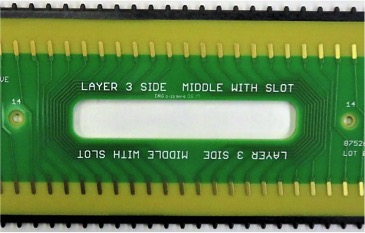
\includegraphics[height=0.28\textheight]{sp-apa-side-board-slot.jpg} \quad
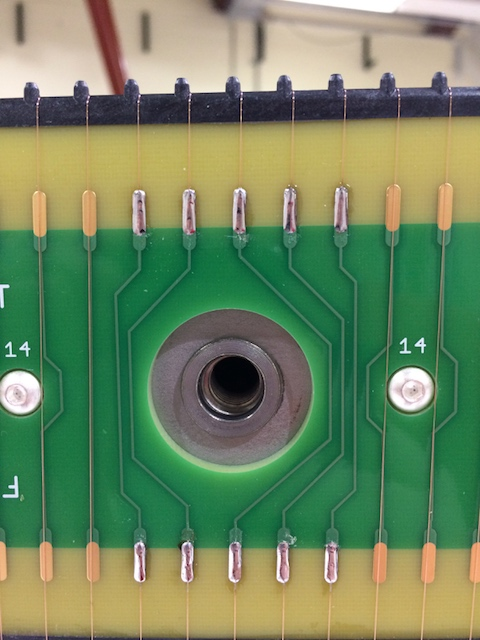
\includegraphics[height=0.28\textheight,trim=0mm 0mm 0mm 25mm,clip]{sp-apa-side-board-round-hole.jpg}
\end{dunefigure}

The placement of the angled wires are fixed by teeth that are part of an injected molded strip glued to the edge of the \frfour boards.  The polymer used for the strips is Vectra e130i (a trade name for 30$\%$ glass filled liquid crystal polymer, or LCP). It retains its strength at cryogenic temperature and has a \dword{cte} similar enough to \frfour that differential contraction is not a problem.  The wires make a partial wrap around the pin as they change direction from the face of the \dword{apa} to the edge.


%%%%%%%%%%%%%%%%%%%%%%%%%%
\subsubsection{Capacitive-Resistive (CR) Boards}
\label{sec:crboards}

The \dword{cr} boards carry a bias resistor and a DC-blocking capacitor for each wire in the $X$ and $U$-planes. These boards are attached to the board stacks after fabrication of all wire planes.   Electrical connections to the board stack are made through Mill-Max pins that plug into the wire boards. Connections from the \dword{cr} boards to the \dword{ce} are made through a pair of \num{96}-pin Samtec\footnote{Samtec\texttrademark \url{https://www.samtec.com/}} connectors.

Surface-mount bias resistors on the \dword{cr} boards have resistance of \SI{50}{\mega\ohm} and are constructed with a thick film on a ceramic substrate. Rated for \SI{2.0}{kV} operation, the resistors measure \SI{3.0 x 6.1}{mm} (\SI{0.12 x 0.24}{in}). The selected DC-blocking capacitors have capacitance of \SI{3.9}{nF} and are rated for \SI{2.0}{kV} operation. Measuring \SI{5.6 x 6.4}{mm} (\SI{0.22 x 0.25}{in}) across and
\SI{2.5}{mm} (\SI{0.10}{in}) high,  
the capacitors feature flexible terminals to comply with \dword{pcb} expansion and contraction. They are designed to withstand \num{1000} thermal cycles between the extremes of the operating temperature range. Tolerance is also \num{5}\,\%.

In addition to the bias and DC-blocking capacitors for all $X$ and $U$-plane wires, the \dword{cr} boards include two R-C filters for the bias voltages\footnote{The $V$-plane does not carry a bias voltage, so does not require these components.}. The resistors are of the same type used for wire biasing except with a resistance of \SI{5}{\mega\ohm}, consisting of two \SI{10}{\mega\ohm} resistors connected in parallel. Wire plane bias filter capacitors are \SI{39}{nF}, consisting of ten \SI{3.9}{nF} surface-mount capacitors connected in parallel. They are the same capacitors as those used for DC blocking.

The selected capacitors were designed by the manufacturer to withstand repeated temperature excursions over a wide range. Their mechanically compliant terminal structure accommodates \dword{cte} mismatches. The resistors use a thick-film technology that is also tolerant of wide temperature excursions.  Capacitors and resistors were qualified for \dword{pdsp} by testing samples repeatedly at room temperature and at \num{-190}\,$^\circ$C.  Performance criteria were measured across five thermal cycles, and no measurable changes were observed. During the production of \num{140} \dword{cr} boards, more than \num{10000} units of each component were tested at room temperature, at \dword{lar} temperature, and again at room temperature. No failures or measurable changes in performance were observed.




%%%%%%%%%%%%%%%%%%%%%%%%%%%%%%%%%%%%%%%
\subsubsection{Support Combs}
\label{sec:combs}

Support combs are glued at four points along each side of the \dword{apa}, along the four cross beams. These combs maintain the wire and plane spacing along the length of the \dword{apa}. A dedicated jig is used to install the combs and also provides the alignment and pressure as the glue dries. The glue used is the Gray epoxy \num{2216} described below. Before the jig can be removed and production can continue, an eight-hour cure time is required after comb installation on each side of the \dword{apa}.  Figure~\ref{fig:tpc_apa_sideboardphoto} shows a detail of the wire support combs on a \dword{pdsp} \dword{apa}.

\begin{dunefigure}[APA side boards on the frame]{fig:tpc_apa_sideboardphoto}
{Left: \dword{apa} corner where end boards meet side boards.  The injection molded teeth that guide the $U$ and $V$ wires around the edge are visible at the bottom. Right: The wire support combs.}
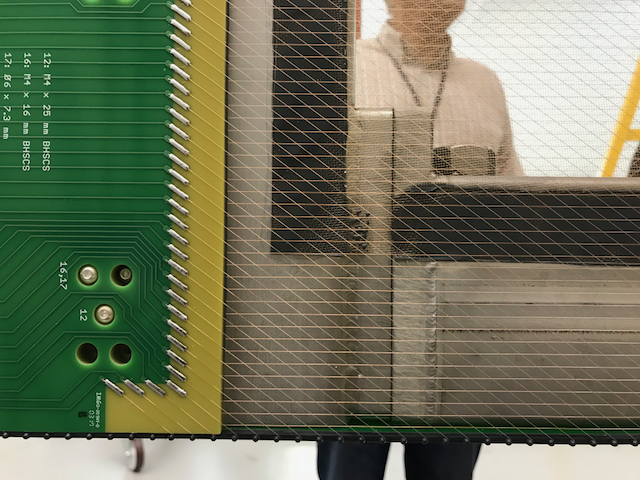
\includegraphics[height=0.32\textheight]{sp-apa-boards-with-pins.png} \quad
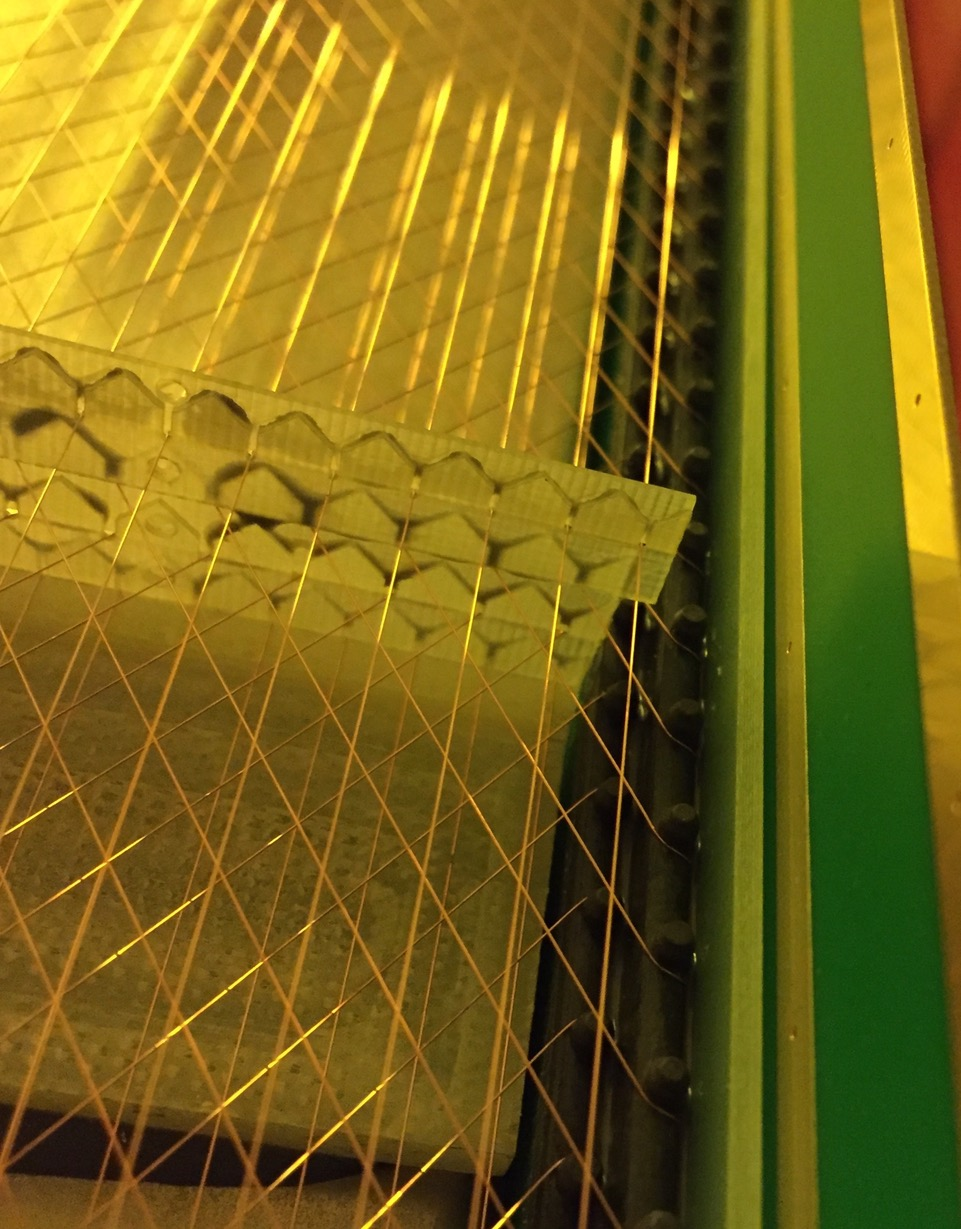
\includegraphics[height=0.32\textheight]{sp-apa-photo-combs.jpg}
\end{dunefigure}

%%%%%%%%%%%%%%%%%%%%%%%%%%%%%%%%%%%%%%%
\subsubsection{Solder and Epoxy}
\label{sec:glue-solder}

The ends of the wires are soldered to pads on the edges of the wire boards.  Solder provides both an electrical connection and a physical anchor to the wire pads. A 62$\%$ tin, 36$\%$ lead, and 2$\%$ silver solder was chosen.  A eutectic mix (63/37) is the best of the straight tin-lead solders, but the 2$\%$ added silver gives better creep resistance.  The solder contains a no-clean flux and does not need to be removed after soldering. Most of it is encapsulated when subsequent boards are epoxied in place.  At room temperatures and below, the flux is not conductive or corrosive.

Once a wire layer is complete, the next layer of boards is glued on; this glue provides an additional physical anchor. Gray epoxy \num{2216} by 3M\footnote{3M\texttrademark ~\url{https://www.3m.com/}} is used for the glue.  It is strong and widely used (therefore much data is available), and it retains good properties at cryogenic temperatures.  



%%%%%%%%%%%%%%%%%%%%%%%%%%%%%%%%%
\subsection{The APA Pair} %Doublet}
\label{sec:fdsp-apa-intfc-apa}


In an \dword{spmod}, pairs of \SI{6}{m} tall \dword{apa} frames are mechanically connected at their ends to form a \SI{12}{m} tall readout surface.  Figure~\ref{fig:apa-doublet} shows a connected pair (turned on its side) with dimensions.  The \dword{tpc} readout electronics require that the individual \dword{apa} frames be electrically isolated.   The left panel of Figure~\ref{fig:apa-connections} shows the design for mechanically connecting \dword{apa}s while maintaining electrical isolation.  The two \dword{apa}s are connected through a stainless steel link that is attached to both frames with a special shoulder screw.  The steel part of the link is electrically insulated from the frames using a G10 panel.  The links connect to the side tubes with a special shoulder screw that screws into plates welded to the frame.  

\begin{dunefigure}[APA pair diagram with dimensions]{fig:apa-doublet}
{Diagram of an \dword{apa} pair, with connected bottom and top \dword{apa}. The dimensions of the \dword{apa} pair, including the accompanying cold electronics and mechanical supports (the yoke), are indicated.}
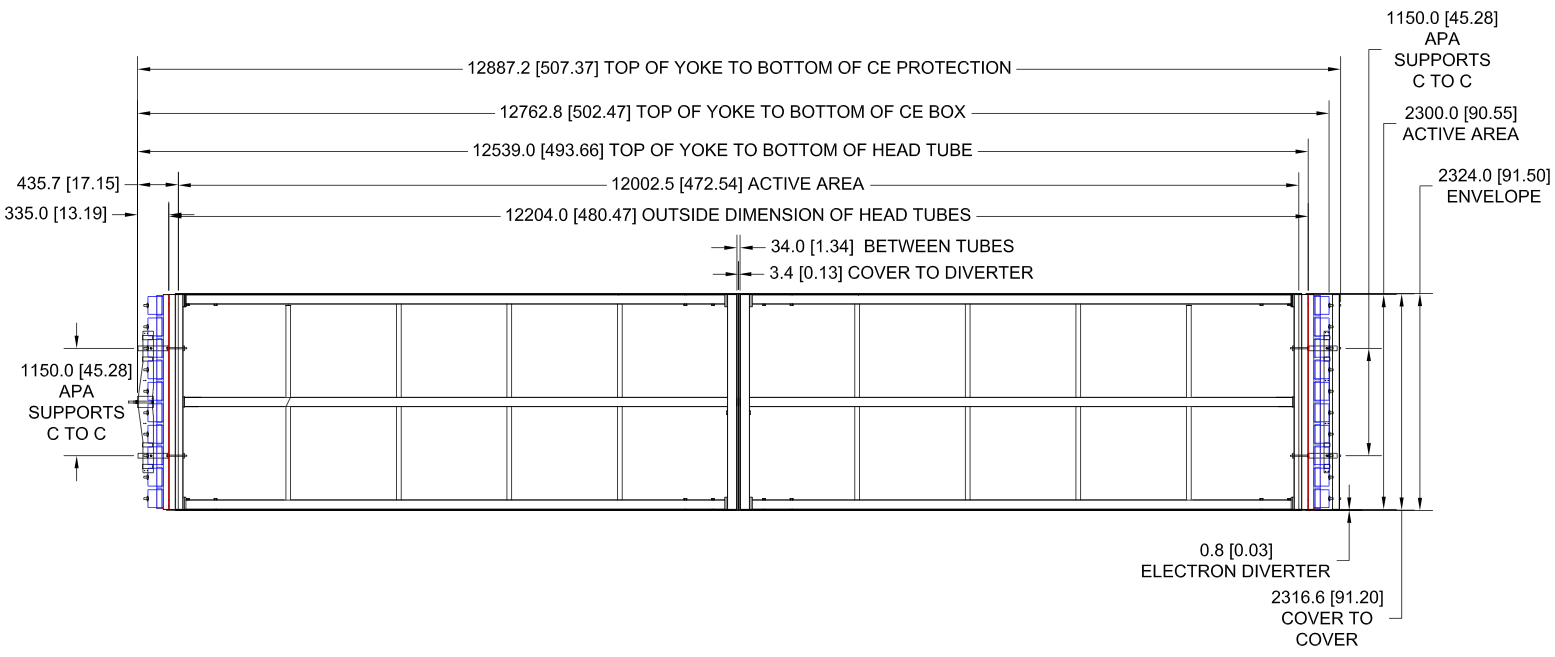
\includegraphics[width=1\textwidth]{sp-apa-stack.jpg} 
\end{dunefigure}

\begin{dunefigure}[APA-to-APA connections]{fig:apa-connections}
{Design for the \dword{apa}-to-\dword{apa} connections.  Left: For the vertical connection there are two steel links joining the upper APA to the lower APA; one link connected to one APA is shown here.  The steel part of the link is electrically insulated from the frames.  Right: Along adjoining vertical edges, two pins keep neighboring \dword{apa}s in plane. Two side tubes before engagement with the screw and insulating sleeve installed are shown at the top, and the engaged side tubes are shown below.}  
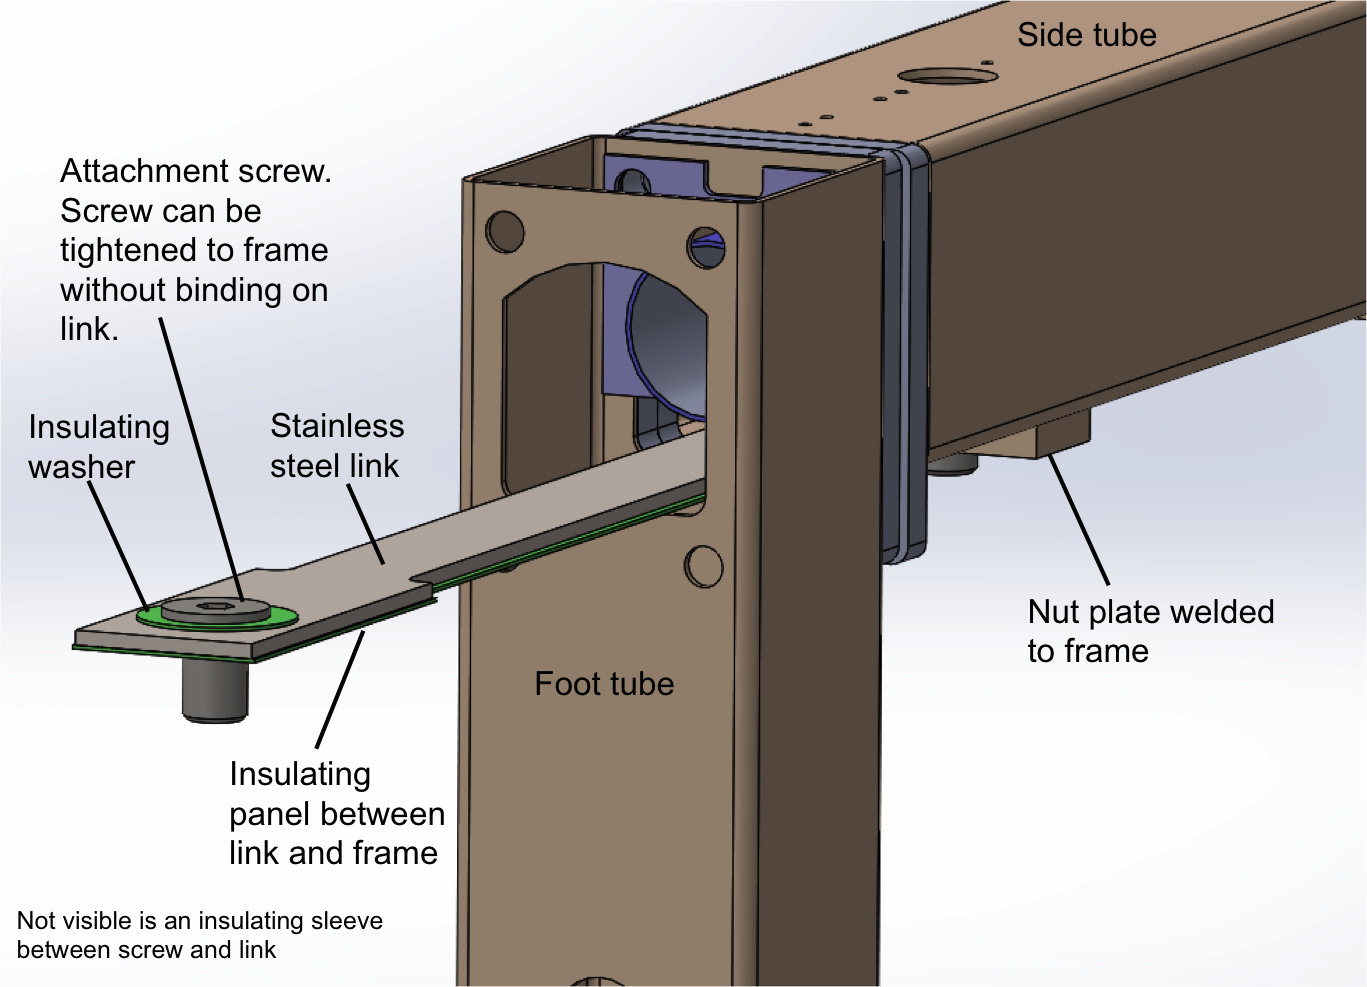
\includegraphics[height=0.29\textheight]{sp-apa-apa-mating-2.png} \qquad
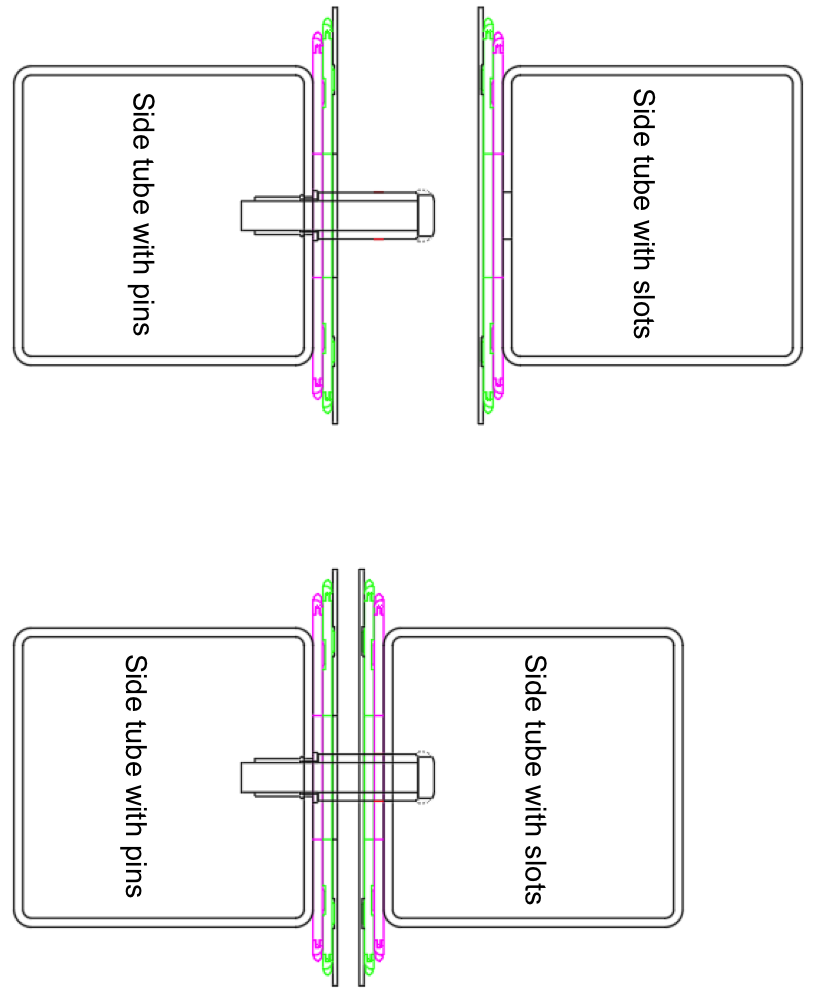
\includegraphics[height=0.3\textheight]{sp-apa-side-mating-2.png}
\end{dunefigure}

The \dword{apa} yoke, shown in Figure~\ref{fig:apa-yoke}, is a bolted stainless steel structural assembly with a central support point and a pair of pins to connect to the load.  Two T-shaped brackets, referred to as the structural tees, mount to the head tube of the top \dword{apa} and provide the mating pin holes to connect the yoke to the \dword{apa}.  The center support point consists of a M20 stainless steel bolt, oversize washers, and a PEEK washer for electrical isolation.   The yoke is mounted to the top \dword{apa} before an \dword{apa} pair %doublet 
is assembled.  To move into the cryostat, the pair %doublet 
is hung from two trolleys that connect to the structural tees. Once in final position, the load of the \dword{apa} pair %doublet 
can be transferred from the trolleys to the \dword{dss} in the cryostat through the center support point of the yoke.  To accomplish this, the M20 bolt and washer assembly is inserted from the bottom of the yoke and the threaded end of the bolt connects to the \dword{dss}.

\begin{dunefigure}[Yoke that connects an APA pair %doublet 
to the DSS]{fig:apa-yoke} % I got rid of doublet in other chaps
{The yoke at the top of an \dword{apa} pair %doublet 
that provides connection to the \dword{dss}.}
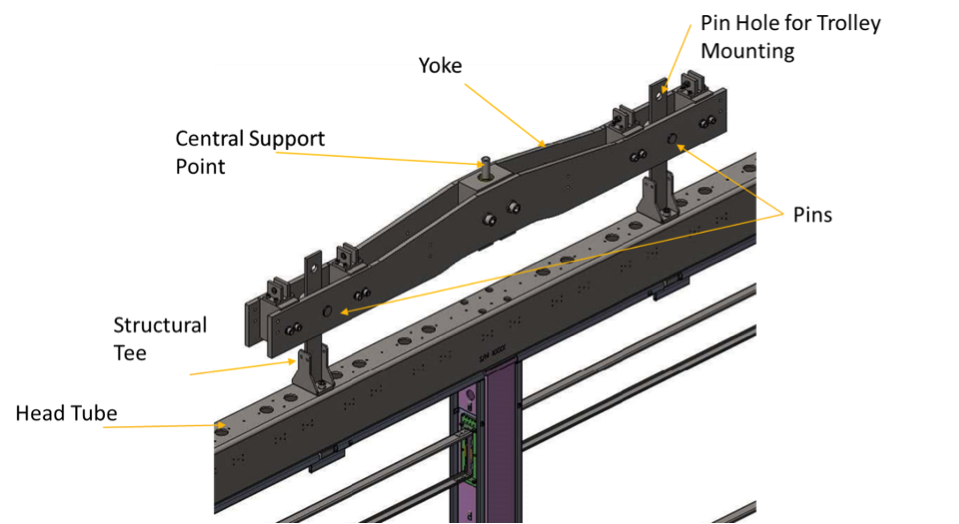
\includegraphics[width=0.95\textwidth]{sp-apa-yoke-labels.png} 
\end{dunefigure}

Adjacent \dword{apa} pairs %doublets 
are kept in plane with each other by simple insertion pins at the top and bottom of the side tubes.  The pins are made up of a screw and an insulating sleeve to ensure electrical isolation, and each pin engages a slot in the adjacent \dword{apa} pair %doublet 
side tubes. The right panel of Figure~\ref{fig:apa-connections} shows a schematic of the side pin connectors before and after insertion.  

Once installed in the detector, a physical gap of \SI{12}{mm} exists along this vertical connection between all adjacent \dword{apa}s at room temperature. Since the \dword{apa}s are suspended under the stainless steel \dword{dss} beams, which contract similarly to that of the \dword{apa} frames, the gaps between most adjacent \dword{apa}s stay about the same (\SI{12}{mm}) in the cold.  The \dword{dss} beams, however, are segmented at \SI{6.4}{m} length, and each beam segment is independently supported by two \dword{dss} feedthroughs, one of which does not allow lateral movement.  As a result, the gaps between \dword{dss} beams open up in the cold by another \SI{17}{mm},  %This additional \SI{17}{mm} needs to be added to the \dword{apa}s spanning the beam boundaries, 
making the physical gaps \SI{29}{mm} as shown in Figure~\ref{fig:sp-apa-gaps}.  The actual gap between the \dword{apa}s active width \SI{28}{mm} is approximately \SI{16}{mm} wider than the physical gap (\SI{45}{mm}) in the two scenarios described above.

\begin{dunefigure}[APA-to-APA gaps]{fig:sp-apa-gaps}
{Illustration of the gap width between \dword{apa}s}  
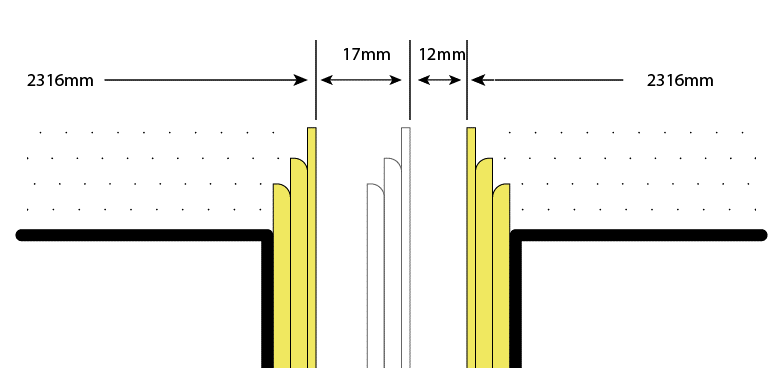
\includegraphics[width=0.8\textwidth]{sp-apa-gaps.png} 
\end{dunefigure}

 
To minimize the loss of signal charge over the gaps between \dword{apa}s in \dword{pdsp}, special electrodes (electron diverters) were installed along the vertical gaps to nudge the incoming electrons into the active regions of the \dword{apa}s. The data from \dword{pdsp} are being used to study the impact of using electron diverters and determine the need for them in \dword{dune}.  See Section~\ref{sec:fdsp-apa-qa} for a discussion of the \dword{pdsp} data analysis (\dword{pdsp} had some gaps with electron diverters installed and some without, enabling comparisons of the tracking and calorimetry performance in the two cases). %The final decision of whether to use electron diverters in \dword{dune} %will be made by the \dword{dune} technical board during summer 2019.    





\subsection{APA Structural Analysis}

The \dword{apa}s will be subjected to a variety of load conditions throughout construction, installation, and operation of the experiment, so it is important to analyze carefully and confirm the design of the mechanical components.  A structural and safety analysis was performed to confirm the strength of the \dword{apa} frame, the \dword{apa} yoke, and the \dword{apa}-to-\dword{apa} link.  The full report can be found at~\cite{bib:cernedms2100877}. %https://edms.cern.ch/document/2100877/1. 
As noted, the way the \dword{apa} frame is supported and loaded changes during the construction and transport of the \dword{apa}. Twenty different load cases were checked.  These load cases cover the handling of the bare frame, the \dword{apa} during wiring, the fully integrated \dword{apa}, and the \dword{apa} pair.  The analysis covered the loaded \dword{apa} pair in the installed warm and dry state as well as spatial and transient thermal gradients that might be encountered during cool down.

The masses of components mounted on the frame were determined from the material densities and the geometry defined in the \threed models.  Loads from the supported masses and the APA wire load were applied to the frame in the analysis to replicate the way loads are applied to the actual frame.  The analysis was performed in accordance with the standard building code for large steel structures, the \dwords{asic} Specification for Structural Steel Buildings (AISC document 360-10). For stainless steel structures, the \dword{asic}  publication Design Guide 27: Structural Stainless Steel was also applied.  The analysis was performed using the Load and Resistance Factor Design method (LRFD).

Per LRFD, a load factor of 1.4 was applied to all loads and to the self-weight of the \dword{apa}  frame.  The factored loads were used to calculate the required strength or stress.  Strength reduction factors were assigned to the strength or stress rating of the component or material.  The strength reduction factors determined the allowable strengths and the design was considered to meet code as long as the allowable strength of the material or component is greater than the required strength as determined by the factored loading.

In order to evaluate the structure, a \dword{fea}  model of the \dword{apa}  frame was built in SolidWorks Simulation\footnote{\url{https://www.solidworks.com/}}.   For each load case, proper constraints were defined and factored loads were applied.  The stress in the frame members were directly extracted from the model.  Also extracted from the model were the forces and moments acting on the welded and bolted joints. These forces and moments and methods from code were used to determine the required strength.  The allowable strength was also determined using methods from the code.
For transportation cases, the analysis was used to determine that the maximum shock or g-load the \dword{apa}  frame can tolerate is 4g (\SI{39.2}{m/s^2}).  This value has been incorporated into the requirements for the design of the transport frame.

Two thermal cases were run. In one case, a steady state thermal gradient of \SI{17}{K/m} was applied to the frame in addition to the installed state loading.   The second thermal case was a transient case.  In this case, the fastest cool down rate the \dword{apa}  frame can tolerate without over stressing the wires and wire solder/epoxy joints was estimated.  The wire cools faster than the frame and the \cooldown rate is limited by a 75~$^\circ$C allowable differential temperature between the frame and the wire.  The estimation of the differential was done using a conservative method that is described in the section that presents the results for case 20 in the \dword{apa} analysis document.  The allowable cool down rate of the ambient environment is 70~$^\circ$C/hr.

In addition to the frame, the yoke was also analyzed for strength.  These components are not subjected to multiple load states and see their maximum loads when in the installed state.  The yoke was analyzed using \dword{fea} to check stress and buckling of the side plates.  The \dword{apa} -to-\dword{apa}  link was checked using methods for pinned connections defined in code.

Results for the frame analysis show the frame members are most heavily stressed in the transportation cases.  This is expected because the g-load was increased until strength limits were reached.  Here the ratio of allowable to required strength is 1.1 for both the beam structural members and for the welds and 1.5 for the bolts.
The results for the yoke analysis show that the allowable stress over the required strength for the yoke plates is 2.2.  The ratio of the load that will cause buckling to the applied load is 33.

The structural analysis clearly shows the \dword{apa}  frame members, welds, and bolts are strong enough to carry the loads.
